% -------------------------------------------------------------------------------- %

\begin{exercise}

Erklären Sie die Funktionsweise der Algorithmen von Kruskal und Prim anhand der Konstruktion eines maximalen Spannbaums (eines spannenden Baums mit maximalen Gewicht) mittels Kruskal's Algorithmus und eines minimalen Spannbaums mittels Prim's Algorithmus für den Wurzelknoten $s$ im folgenden kantenbewerteten Graph:

\begin{center}
    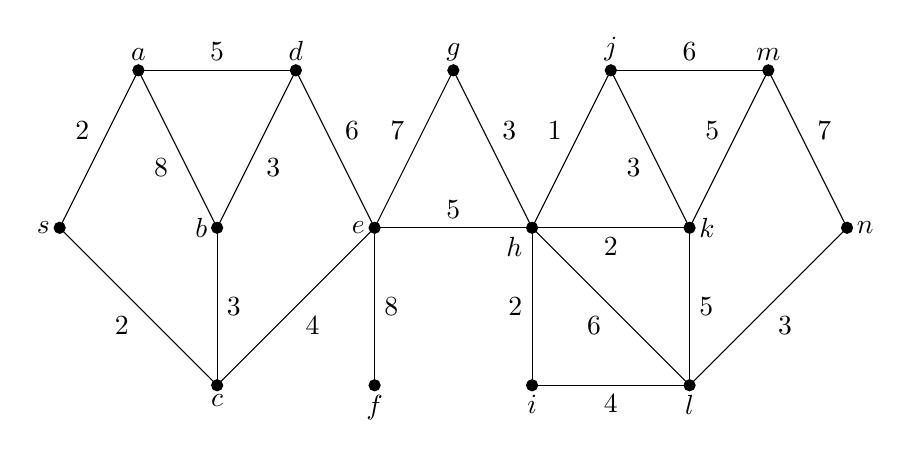
\begin{tikzpicture}

    \coordinate (a) at ( 1, 4);
\coordinate (b) at ( 2, 2);
\coordinate (c) at ( 2, 0);
\coordinate (d) at ( 3, 4);
\coordinate (e) at ( 4, 2);
\coordinate (f) at ( 4, 0);
\coordinate (g) at ( 5, 4);
\coordinate (h) at ( 6, 2);
\coordinate (i) at ( 6, 0);
\coordinate (j) at ( 7, 4);
\coordinate (k) at ( 8, 2);
\coordinate (l) at ( 8, 0);
\coordinate (m) at ( 9, 4);
\coordinate (n) at (10, 2);
\coordinate (s) at ( 0, 2);

    \draw [color = black] (a) -- node [below left]  {$8$} (b);
    \draw [color = black] (a) -- node [above]       {$5$} (d);
    \draw [color = black] (a) -- node [above left]  {$2$} (s);
    \draw [color = black] (b) -- node [right]       {$3$} (c);
    \draw [color = black] (b) -- node [below right] {$3$} (d);
    \draw [color = black] (c) -- node [below right] {$4$} (e);
    \draw [color = black] (c) -- node [below left]  {$2$} (s);
    \draw [color = black] (d) -- node [above right] {$6$} (e);
    \draw [color = black] (e) -- node [right]       {$8$} (f);
    \draw [color = black] (e) -- node [above left]  {$7$} (g);
    \draw [color = black] (e) -- node [above]       {$5$} (h);
    \draw [color = black] (g) -- node [above right] {$3$} (h);
    \draw [color = black] (h) -- node [left]        {$2$} (i);
    \draw [color = black] (h) -- node [above left]  {$1$} (j);
    \draw [color = black] (h) -- node [below]       {$2$} (k);
    \draw [color = black] (h) -- node [below left]  {$6$} (l);
    \draw [color = black] (i) -- node [below]       {$4$} (l);
    \draw [color = black] (j) -- node [below left]  {$3$} (k);
    \draw [color = black] (j) -- node [above]       {$6$} (m);
    \draw [color = black] (k) -- node [right]       {$5$} (l);
    \draw [color = black] (k) -- node [above left]  {$5$} (m);
    \draw [color = black] (l) -- node [below right] {$3$} (n);
    \draw [color = black] (m) -- node [above right] {$7$} (n);

    \filldraw [color = black] (a) circle (2pt) node [above]      {$a$};
    \filldraw [color = black] (b) circle (2pt) node [left]       {$b$};
    \filldraw [color = black] (c) circle (2pt) node [below]      {$c$};
    \filldraw [color = black] (d) circle (2pt) node [above]      {$d$};
    \filldraw [color = black] (e) circle (2pt) node [left]       {$e$};
    \filldraw [color = black] (f) circle (2pt) node [below]      {$f$};
    \filldraw [color = black] (g) circle (2pt) node [above]      {$g$};
    \filldraw [color = black] (h) circle (2pt) node [below left] {$h$};
    \filldraw [color = black] (i) circle (2pt) node [below]      {$i$};
    \filldraw [color = black] (j) circle (2pt) node [above]      {$j$};
    \filldraw [color = black] (k) circle (2pt) node [right]      {$k$};
    \filldraw [color = black] (l) circle (2pt) node [below]      {$l$};
    \filldraw [color = black] (m) circle (2pt) node [above]      {$m$};
    \filldraw [color = black] (n) circle (2pt) node [right]      {$n$};
    \filldraw [color = black] (s) circle (2pt) node [left]       {$s$};

\end{tikzpicture}

\end{center}

% \begin{center}
%     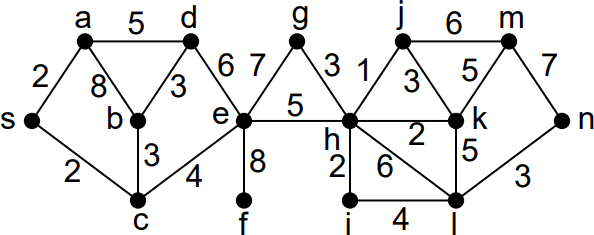
\includegraphics[width = 0.5 \textwidth]{7.38.png}
% \end{center}

\end{exercise}

% -------------------------------------------------------------------------------- %

\begin{solution}

\phantom{}

\begin{enumerate}[label = \arabic*.]

    \item Algorithmus (von Kruskal):

    Der Algorithmus von Kruskal erhält als Eingabe einen zusammenhängenden endlichen (möglicherweise sogar gerichteten) Graphen $G = (V, E)$ und eine Kostenfunktion $c: E  \to \R^+$.

    \begin{align*}
        G = (V, E),
        \quad
        V = \Bbraces{a, b, c, d, e, f, g, h, i, j, k, l, m, n, s},
    \end{align*}

    \begin{multline*}
        E =
        \{
            \Bbraces{a, b},
            \Bbraces{a, d},
            \Bbraces{a, s},
            \Bbraces{b, c},
            \Bbraces{b, d},
            \Bbraces{c, e},
            \Bbraces{c, s},
            \Bbraces{d, e},
            \Bbraces{e, f},
            \Bbraces{e, g},
            \Bbraces{e, h}, \\
            \Bbraces{g, h},
            \Bbraces{h, i},
            \Bbraces{h, j},
            \Bbraces{h, k},
            \Bbraces{h, l},
            \Bbraces{i, l},
            \Bbraces{j, k},
            \Bbraces{j, m},
            \Bbraces{k, l},
            \Bbraces{k, m},
            \Bbraces{l, n},
            \Bbraces{m, n}
        \}
    \end{multline*}

    \begin{align*}
        \begin{matrix}
            c(\Bbraces{a, b}) = 8, & c(\Bbraces{a, d}) = 5, & c(\Bbraces{a, s}) = 2, & \\
            c(\Bbraces{b, c}) = 3, & c(\Bbraces{b, d}) = 3, & & \\
            c(\Bbraces{c, e}) = 4, & c(\Bbraces{c, s}) = 2, & & \\
            c(\Bbraces{d, e}) = 6, & & & \\
            c(\Bbraces{e, f}) = 8, & c(\Bbraces{e, g}) = 7, & c(\Bbraces{e, h}) = 5, & \\
            c(\Bbraces{g, h}) = 3, & & & \\
            c(\Bbraces{h, i}) = 2, & c(\Bbraces{h, j}) = 1, & c(\Bbraces{h, k}) = 2, & c(\Bbraces{h, l}) = 6, \\
            c(\Bbraces{i, l}) = 4, & & & \\
            c(\Bbraces{j, k}) = 3, & c(\Bbraces{j, m}) = 6, & & \\
            c(\Bbraces{k, l}) = 5, & c(\Bbraces{k, m}) = 5, & & \\
            c(\Bbraces{l, n}) = 3, & & & \\
            c(\Bbraces{m, n}) = 7  & & &
        \end{matrix}
    \end{align*}

    $B$ wird die Kanten-Menge des gewünschten minimalen Spannbaums von $G$.
    Diese startet mit der leeren Menge $\emptyset$ und es werden sukzessive passende Kanten hinzugefügt.

    Zuerst wird allerdings der Graph in einen Wald $P$ aus $1$-punktigen Bäumen partitioniert.

    \begin{multline*}
        P_0
        :=
        \{
            (\Bbraces{a}, \emptyset),
            (\Bbraces{b}, \emptyset),
            (\Bbraces{c}, \emptyset),
            (\Bbraces{d}, \emptyset),
            (\Bbraces{e}, \emptyset),
            (\Bbraces{f}, \emptyset),
            (\Bbraces{g}, \emptyset), \\
            (\Bbraces{h}, \emptyset),
            (\Bbraces{i}, \emptyset),
            (\Bbraces{j}, \emptyset),
            (\Bbraces{k}, \emptyset),
            (\Bbraces{l}, \emptyset),
            (\Bbraces{m}, \emptyset),
            (\Bbraces{n}, \emptyset),
            (\Bbraces{s}, \emptyset)
        \}
    \end{multline*}

    Diese Bäume werden mit passenden Kanten $\in E$ zu einem minimalen Spannbaum verknüpft.
    Dazu iteriert man über das aus $E$ bzgl. $c$ von oben nach unten sortierte Datenfeld.

    \begin{align*}
        \begin{matrix}
            c(\Bbraces{a, b}) = 8 & \geq & c(\Bbraces{e, f}) = 8 & \geq &                       &      &                       &      &                       &      \\
            c(\Bbraces{e, g}) = 7 & \geq & c(\Bbraces{m, n}) = 7 & \geq &                       &      &                       &      &                       &      \\
            c(\Bbraces{d, e}) = 6 & \geq & c(\Bbraces{h, l}) = 6 & \geq & c(\Bbraces{j, m}) = 6 & \geq &                       &      &                       &      \\
            c(\Bbraces{a, d}) = 5 & \geq & c(\Bbraces{e, h}) = 5 & \geq & c(\Bbraces{k, l}) = 5 & \geq & c(\Bbraces{k, m}) = 5 & \geq &                       &      \\
            c(\Bbraces{c, e}) = 4 & \geq & c(\Bbraces{i, l}) = 4 & \geq &                       &      &                       &      &                       &      \\
            c(\Bbraces{b, c}) = 3 & \geq & c(\Bbraces{b, d}) = 3 & \geq & c(\Bbraces{g, h}) = 3 & \geq & c(\Bbraces{j, k}) = 3 & \geq & c(\Bbraces{l, n}) = 3 & \geq \\
            c(\Bbraces{a, s}) = 2 & \geq & c(\Bbraces{c, s}) = 2 & \geq & c(\Bbraces{h, i}) = 2 & \geq & c(\Bbraces{h, k}) = 2 & \geq &                       &      \\
            c(\Bbraces{h, j}) = 1 &      &                       &      &                       &      &                       &      &                       &
        \end{matrix}
    \end{align*}

    \begin{multline*}
        E \mapsto
        [
            \Bbraces{a, b},
            \Bbraces{e, f},
            \Bbraces{e, g},
            \Bbraces{m, n},
            \Bbraces{d, e},
            \Bbraces{h, l},
            \Bbraces{j, m},
            \Bbraces{a, d},
            \Bbraces{e, h},
            \Bbraces{k, l},
            \Bbraces{k, m}, \\
            \Bbraces{c, e},
            \Bbraces{i, l},
            \Bbraces{b, c},
            \Bbraces{b, d},
            \Bbraces{g, h},
            \Bbraces{j, k},
            \Bbraces{l, n},
            \Bbraces{a, s},
            \Bbraces{c, s},
            \Bbraces{h, i},
            \Bbraces{h, k},
            \Bbraces{h, j}
        ]
    \end{multline*}

    Es werden also am ehesten jene Kanten als Verknüpfung verwendet, die maximale Kosten liefern.
    Wir führen exemplarisch ein paar Schritte durch, sodass alle ($2$) Fälle abgedeckt sind.

    \begin{center}
        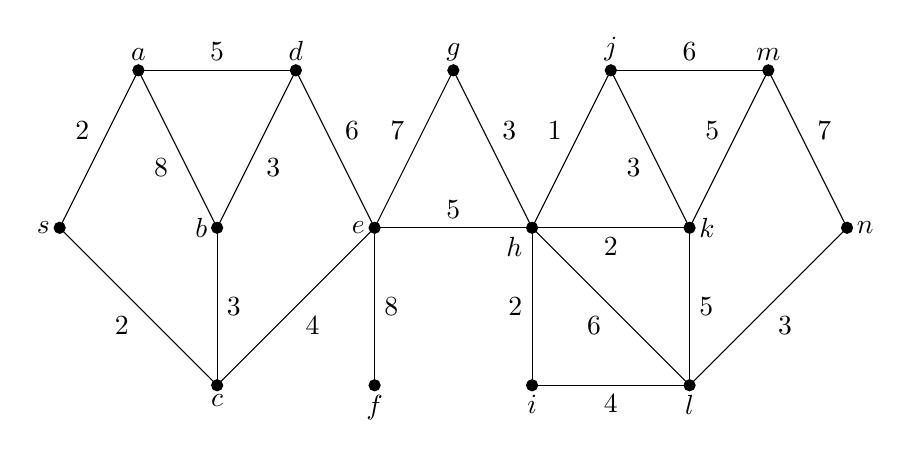
\begin{tikzpicture}

    \coordinate (a) at ( 1, 4);
\coordinate (b) at ( 2, 2);
\coordinate (c) at ( 2, 0);
\coordinate (d) at ( 3, 4);
\coordinate (e) at ( 4, 2);
\coordinate (f) at ( 4, 0);
\coordinate (g) at ( 5, 4);
\coordinate (h) at ( 6, 2);
\coordinate (i) at ( 6, 0);
\coordinate (j) at ( 7, 4);
\coordinate (k) at ( 8, 2);
\coordinate (l) at ( 8, 0);
\coordinate (m) at ( 9, 4);
\coordinate (n) at (10, 2);
\coordinate (s) at ( 0, 2);

    \draw [color = black] (a) -- node [below left]  {$8$} (b);
    \draw [color = black] (a) -- node [above]       {$5$} (d);
    \draw [color = black] (a) -- node [above left]  {$2$} (s);
    \draw [color = black] (b) -- node [right]       {$3$} (c);
    \draw [color = black] (b) -- node [below right] {$3$} (d);
    \draw [color = black] (c) -- node [below right] {$4$} (e);
    \draw [color = black] (c) -- node [below left]  {$2$} (s);
    \draw [color = black] (d) -- node [above right] {$6$} (e);
    \draw [color = black] (e) -- node [right]       {$8$} (f);
    \draw [color = black] (e) -- node [above left]  {$7$} (g);
    \draw [color = black] (e) -- node [above]       {$5$} (h);
    \draw [color = black] (g) -- node [above right] {$3$} (h);
    \draw [color = black] (h) -- node [left]        {$2$} (i);
    \draw [color = black] (h) -- node [above left]  {$1$} (j);
    \draw [color = black] (h) -- node [below]       {$2$} (k);
    \draw [color = black] (h) -- node [below left]  {$6$} (l);
    \draw [color = black] (i) -- node [below]       {$4$} (l);
    \draw [color = black] (j) -- node [below left]  {$3$} (k);
    \draw [color = black] (j) -- node [above]       {$6$} (m);
    \draw [color = black] (k) -- node [right]       {$5$} (l);
    \draw [color = black] (k) -- node [above left]  {$5$} (m);
    \draw [color = black] (l) -- node [below right] {$3$} (n);
    \draw [color = black] (m) -- node [above right] {$7$} (n);

    \filldraw [color = black] (a) circle (2pt) node [above]      {$a$};
    \filldraw [color = black] (b) circle (2pt) node [left]       {$b$};
    \filldraw [color = black] (c) circle (2pt) node [below]      {$c$};
    \filldraw [color = black] (d) circle (2pt) node [above]      {$d$};
    \filldraw [color = black] (e) circle (2pt) node [left]       {$e$};
    \filldraw [color = black] (f) circle (2pt) node [below]      {$f$};
    \filldraw [color = black] (g) circle (2pt) node [above]      {$g$};
    \filldraw [color = black] (h) circle (2pt) node [below left] {$h$};
    \filldraw [color = black] (i) circle (2pt) node [below]      {$i$};
    \filldraw [color = black] (j) circle (2pt) node [above]      {$j$};
    \filldraw [color = black] (k) circle (2pt) node [right]      {$k$};
    \filldraw [color = black] (l) circle (2pt) node [below]      {$l$};
    \filldraw [color = black] (m) circle (2pt) node [above]      {$m$};
    \filldraw [color = black] (n) circle (2pt) node [right]      {$n$};
    \filldraw [color = black] (s) circle (2pt) node [left]       {$s$};

\end{tikzpicture}

    \end{center}

    \begin{multline*}
        P_0
        \stackrel
        {
            \Bbraces{a, b}
        }{
            \mapsto
        }
        P_1 :=
        \{
            (\Bbraces{a, b}, \Bbraces{\Bbraces{a, b}}),
            (\Bbraces{c}, \emptyset),
            (\Bbraces{d}, \emptyset),
            (\Bbraces{e}, \emptyset),
            (\Bbraces{f}, \emptyset),
            (\Bbraces{g}, \emptyset), \\
            (\Bbraces{h}, \emptyset),
            (\Bbraces{i}, \emptyset),
            (\Bbraces{j}, \emptyset),
            (\Bbraces{k}, \emptyset),
            (\Bbraces{l}, \emptyset),
            (\Bbraces{m}, \emptyset),
            (\Bbraces{n}, \emptyset),
            (\Bbraces{s}, \emptyset)
        \}
    \end{multline*}

    \begin{center}
        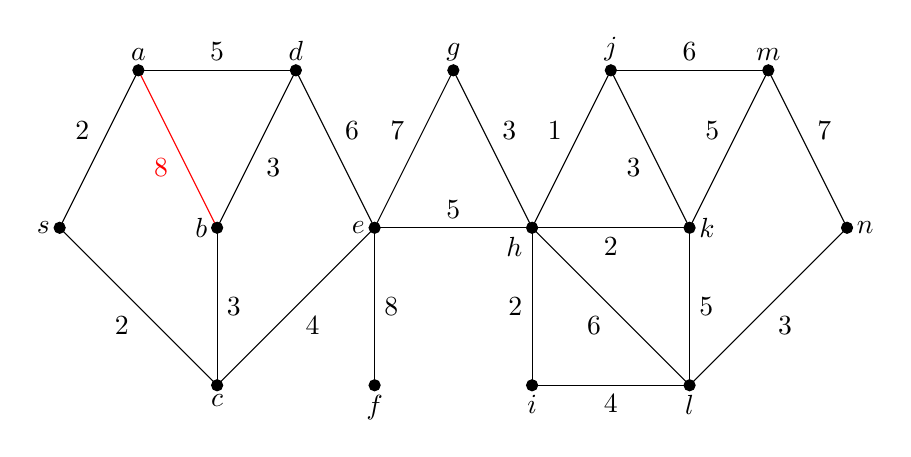
\begin{tikzpicture}

    \coordinate (a) at ( 1, 4);
\coordinate (b) at ( 2, 2);
\coordinate (c) at ( 2, 0);
\coordinate (d) at ( 3, 4);
\coordinate (e) at ( 4, 2);
\coordinate (f) at ( 4, 0);
\coordinate (g) at ( 5, 4);
\coordinate (h) at ( 6, 2);
\coordinate (i) at ( 6, 0);
\coordinate (j) at ( 7, 4);
\coordinate (k) at ( 8, 2);
\coordinate (l) at ( 8, 0);
\coordinate (m) at ( 9, 4);
\coordinate (n) at (10, 2);
\coordinate (s) at ( 0, 2);

    \draw [color = red] (a) -- node [below left]  {$8$} (b);
    \draw [color = black] (a) -- node [above]       {$5$} (d);
    \draw [color = black] (a) -- node [above left]  {$2$} (s);
    \draw [color = black] (b) -- node [right]       {$3$} (c);
    \draw [color = black] (b) -- node [below right] {$3$} (d);
    \draw [color = black] (c) -- node [below right] {$4$} (e);
    \draw [color = black] (c) -- node [below left]  {$2$} (s);
    \draw [color = black] (d) -- node [above right] {$6$} (e);
    \draw [color = black] (e) -- node [right]       {$8$} (f);
    \draw [color = black] (e) -- node [above left]  {$7$} (g);
    \draw [color = black] (e) -- node [above]       {$5$} (h);
    \draw [color = black] (g) -- node [above right] {$3$} (h);
    \draw [color = black] (h) -- node [left]        {$2$} (i);
    \draw [color = black] (h) -- node [above left]  {$1$} (j);
    \draw [color = black] (h) -- node [below]       {$2$} (k);
    \draw [color = black] (h) -- node [below left]  {$6$} (l);
    \draw [color = black] (i) -- node [below]       {$4$} (l);
    \draw [color = black] (j) -- node [below left]  {$3$} (k);
    \draw [color = black] (j) -- node [above]       {$6$} (m);
    \draw [color = black] (k) -- node [right]       {$5$} (l);
    \draw [color = black] (k) -- node [above left]  {$5$} (m);
    \draw [color = black] (l) -- node [below right] {$3$} (n);
    \draw [color = black] (m) -- node [above right] {$7$} (n);

    \filldraw [color = black] (a) circle (2pt) node [above]      {$a$};
    \filldraw [color = black] (b) circle (2pt) node [left]       {$b$};
    \filldraw [color = black] (c) circle (2pt) node [below]      {$c$};
    \filldraw [color = black] (d) circle (2pt) node [above]      {$d$};
    \filldraw [color = black] (e) circle (2pt) node [left]       {$e$};
    \filldraw [color = black] (f) circle (2pt) node [below]      {$f$};
    \filldraw [color = black] (g) circle (2pt) node [above]      {$g$};
    \filldraw [color = black] (h) circle (2pt) node [below left] {$h$};
    \filldraw [color = black] (i) circle (2pt) node [below]      {$i$};
    \filldraw [color = black] (j) circle (2pt) node [above]      {$j$};
    \filldraw [color = black] (k) circle (2pt) node [right]      {$k$};
    \filldraw [color = black] (l) circle (2pt) node [below]      {$l$};
    \filldraw [color = black] (m) circle (2pt) node [above]      {$m$};
    \filldraw [color = black] (n) circle (2pt) node [right]      {$n$};
    \filldraw [color = black]   (s) circle (2pt) node [left]       {$s$};

\end{tikzpicture}

    \end{center}

    \begin{multline*}
        P_1
        \stackrel
        {
            \Bbraces{e, f}
        }{
            \mapsto
        }
        P_2 :=
        \{
            (\Bbraces{a, b}, \Bbraces{\Bbraces{a, b}}),
            (\Bbraces{c}, \emptyset),
            (\Bbraces{d}, \emptyset),
            (\Bbraces{e, f}, \Bbraces{\Bbraces{e, f}}),
            (\Bbraces{g}, \emptyset), \\
            (\Bbraces{h}, \emptyset),
            (\Bbraces{i}, \emptyset),
            (\Bbraces{j}, \emptyset),
            (\Bbraces{k}, \emptyset),
            (\Bbraces{l}, \emptyset),
            (\Bbraces{m}, \emptyset),
            (\Bbraces{n}, \emptyset),
            (\Bbraces{s}, \emptyset)
        \}
    \end{multline*}

    \begin{center}
        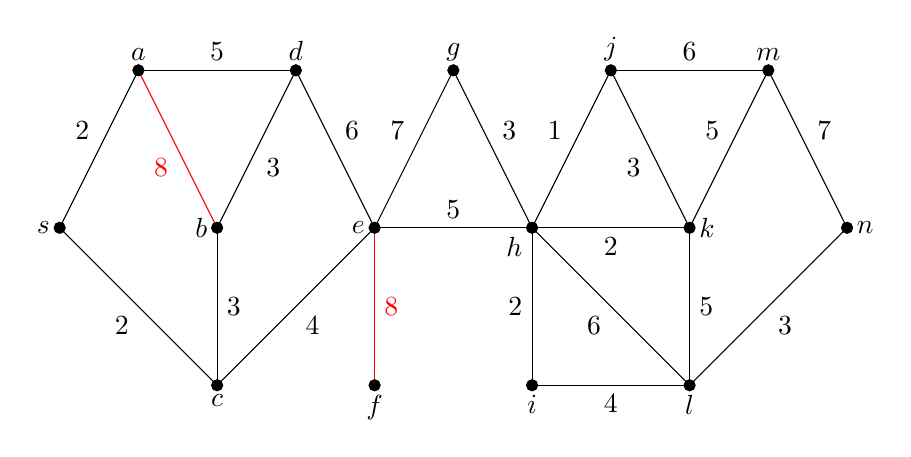
\begin{tikzpicture}

    \coordinate (a) at ( 1, 4);
\coordinate (b) at ( 2, 2);
\coordinate (c) at ( 2, 0);
\coordinate (d) at ( 3, 4);
\coordinate (e) at ( 4, 2);
\coordinate (f) at ( 4, 0);
\coordinate (g) at ( 5, 4);
\coordinate (h) at ( 6, 2);
\coordinate (i) at ( 6, 0);
\coordinate (j) at ( 7, 4);
\coordinate (k) at ( 8, 2);
\coordinate (l) at ( 8, 0);
\coordinate (m) at ( 9, 4);
\coordinate (n) at (10, 2);
\coordinate (s) at ( 0, 2);

    \draw [color = red] (a) -- node [below left]  {$8$} (b);
    \draw [color = black] (a) -- node [above]       {$5$} (d);
    \draw [color = black] (a) -- node [above left]  {$2$} (s);
    \draw [color = black] (b) -- node [right]       {$3$} (c);
    \draw [color = black] (b) -- node [below right] {$3$} (d);
    \draw [color = black] (c) -- node [below right] {$4$} (e);
    \draw [color = black] (c) -- node [below left]  {$2$} (s);
    \draw [color = black] (d) -- node [above right] {$6$} (e);
    \draw [color = red] (e) -- node [right]       {$8$} (f);
    \draw [color = black] (e) -- node [above left]  {$7$} (g);
    \draw [color = black] (e) -- node [above]       {$5$} (h);
    \draw [color = black] (g) -- node [above right] {$3$} (h);
    \draw [color = black] (h) -- node [left]        {$2$} (i);
    \draw [color = black] (h) -- node [above left]  {$1$} (j);
    \draw [color = black] (h) -- node [below]       {$2$} (k);
    \draw [color = black] (h) -- node [below left]  {$6$} (l);
    \draw [color = black] (i) -- node [below]       {$4$} (l);
    \draw [color = black] (j) -- node [below left]  {$3$} (k);
    \draw [color = black] (j) -- node [above]       {$6$} (m);
    \draw [color = black] (k) -- node [right]       {$5$} (l);
    \draw [color = black] (k) -- node [above left]  {$5$} (m);
    \draw [color = black] (l) -- node [below right] {$3$} (n);
    \draw [color = black] (m) -- node [above right] {$7$} (n);

    \filldraw [color = black] (a) circle (2pt) node [above]      {$a$};
    \filldraw [color = black] (b) circle (2pt) node [left]       {$b$};
    \filldraw [color = black] (c) circle (2pt) node [below]      {$c$};
    \filldraw [color = black] (d) circle (2pt) node [above]      {$d$};
    \filldraw [color = black] (e) circle (2pt) node [left]       {$e$};
    \filldraw [color = black] (f) circle (2pt) node [below]      {$f$};
    \filldraw [color = black] (g) circle (2pt) node [above]      {$g$};
    \filldraw [color = black] (h) circle (2pt) node [below left] {$h$};
    \filldraw [color = black] (i) circle (2pt) node [below]      {$i$};
    \filldraw [color = black] (j) circle (2pt) node [above]      {$j$};
    \filldraw [color = black] (k) circle (2pt) node [right]      {$k$};
    \filldraw [color = black] (l) circle (2pt) node [below]      {$l$};
    \filldraw [color = black] (m) circle (2pt) node [above]      {$m$};
    \filldraw [color = black] (n) circle (2pt) node [right]      {$n$};
    \filldraw [color = black]   (s) circle (2pt) node [left]       {$s$};

\end{tikzpicture}

    \end{center}

    \begin{multline*}
        P_2
        \stackrel
        {
            \Bbraces{e, g}
        }{
            \mapsto
        }
        P_3 :=
        \{
            (\Bbraces{a, b}, \Bbraces{\Bbraces{a, b}}),
            (\Bbraces{c}, \emptyset),
            (\Bbraces{d}, \emptyset),
            (\Bbraces{e, f, g}, \Bbraces{\Bbraces{e, f}, \Bbraces{e, g}}), \\
            (\Bbraces{h}, \emptyset),
            (\Bbraces{i}, \emptyset),
            (\Bbraces{j}, \emptyset),
            (\Bbraces{k}, \emptyset),
            (\Bbraces{l}, \emptyset),
            (\Bbraces{m}, \emptyset),
            (\Bbraces{n}, \emptyset),
            (\Bbraces{s}, \emptyset)
        \}
    \end{multline*}

    \begin{center}
        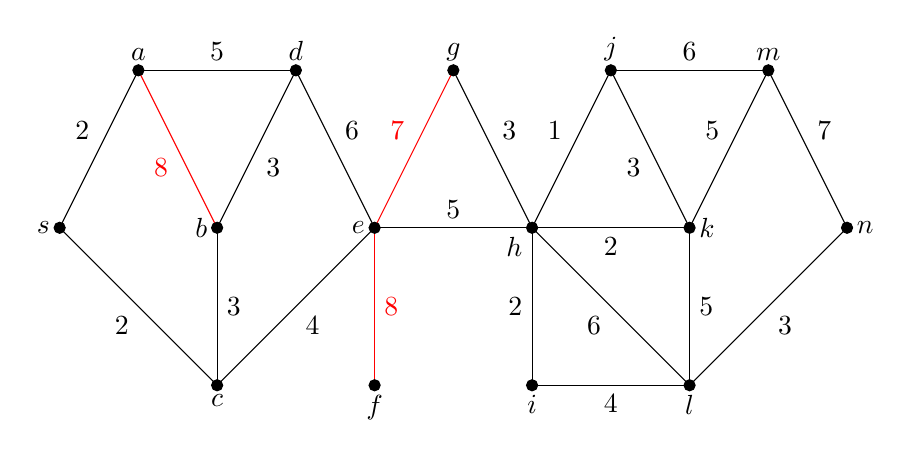
\begin{tikzpicture}

    \coordinate (a) at ( 1, 4);
\coordinate (b) at ( 2, 2);
\coordinate (c) at ( 2, 0);
\coordinate (d) at ( 3, 4);
\coordinate (e) at ( 4, 2);
\coordinate (f) at ( 4, 0);
\coordinate (g) at ( 5, 4);
\coordinate (h) at ( 6, 2);
\coordinate (i) at ( 6, 0);
\coordinate (j) at ( 7, 4);
\coordinate (k) at ( 8, 2);
\coordinate (l) at ( 8, 0);
\coordinate (m) at ( 9, 4);
\coordinate (n) at (10, 2);
\coordinate (s) at ( 0, 2);

    \draw [color = red] (a) -- node [below left]  {$8$} (b);
    \draw [color = black] (a) -- node [above]       {$5$} (d);
    \draw [color = black] (a) -- node [above left]  {$2$} (s);
    \draw [color = black] (b) -- node [right]       {$3$} (c);
    \draw [color = black] (b) -- node [below right] {$3$} (d);
    \draw [color = black] (c) -- node [below right] {$4$} (e);
    \draw [color = black] (c) -- node [below left]  {$2$} (s);
    \draw [color = black] (d) -- node [above right] {$6$} (e);
    \draw [color = red] (e) -- node [right]       {$8$} (f);
    \draw [color = red] (e) -- node [above left]  {$7$} (g);
    \draw [color = black] (e) -- node [above]       {$5$} (h);
    \draw [color = black] (g) -- node [above right] {$3$} (h);
    \draw [color = black] (h) -- node [left]        {$2$} (i);
    \draw [color = black] (h) -- node [above left]  {$1$} (j);
    \draw [color = black] (h) -- node [below]       {$2$} (k);
    \draw [color = black] (h) -- node [below left]  {$6$} (l);
    \draw [color = black] (i) -- node [below]       {$4$} (l);
    \draw [color = black] (j) -- node [below left]  {$3$} (k);
    \draw [color = black] (j) -- node [above]       {$6$} (m);
    \draw [color = black] (k) -- node [right]       {$5$} (l);
    \draw [color = black] (k) -- node [above left]  {$5$} (m);
    \draw [color = black] (l) -- node [below right] {$3$} (n);
    \draw [color = black] (m) -- node [above right] {$7$} (n);

    \filldraw [color = black] (a) circle (2pt) node [above]      {$a$};
    \filldraw [color = black] (b) circle (2pt) node [left]       {$b$};
    \filldraw [color = black] (c) circle (2pt) node [below]      {$c$};
    \filldraw [color = black] (d) circle (2pt) node [above]      {$d$};
    \filldraw [color = black] (e) circle (2pt) node [left]       {$e$};
    \filldraw [color = black] (f) circle (2pt) node [below]      {$f$};
    \filldraw [color = black] (g) circle (2pt) node [above]      {$g$};
    \filldraw [color = black] (h) circle (2pt) node [below left] {$h$};
    \filldraw [color = black] (i) circle (2pt) node [below]      {$i$};
    \filldraw [color = black] (j) circle (2pt) node [above]      {$j$};
    \filldraw [color = black] (k) circle (2pt) node [right]      {$k$};
    \filldraw [color = black] (l) circle (2pt) node [below]      {$l$};
    \filldraw [color = black] (m) circle (2pt) node [above]      {$m$};
    \filldraw [color = black] (n) circle (2pt) node [right]      {$n$};
    \filldraw [color = black]   (s) circle (2pt) node [left]       {$s$};

\end{tikzpicture}

    \end{center}

    \begin{multline*}
        P_3
        \stackrel
        {
            \Bbraces{m, n}
        }{
            \mapsto
        }
        P_4 :=
        \{
            (\Bbraces{a, b}, \Bbraces{\Bbraces{a, b}}),
            (\Bbraces{c}, \emptyset),
            (\Bbraces{d}, \emptyset),
            (\Bbraces{e, f, g}, \Bbraces{\Bbraces{e, f}, \Bbraces{e, g}}), \\
            (\Bbraces{h}, \emptyset),
            (\Bbraces{i}, \emptyset),
            (\Bbraces{j}, \emptyset),
            (\Bbraces{k}, \emptyset),
            (\Bbraces{l}, \emptyset),
            (\Bbraces{m, n}, \Bbraces{\Bbraces{m, n}}),
            (\Bbraces{s}, \emptyset)
        \}
    \end{multline*}

    \begin{center}
        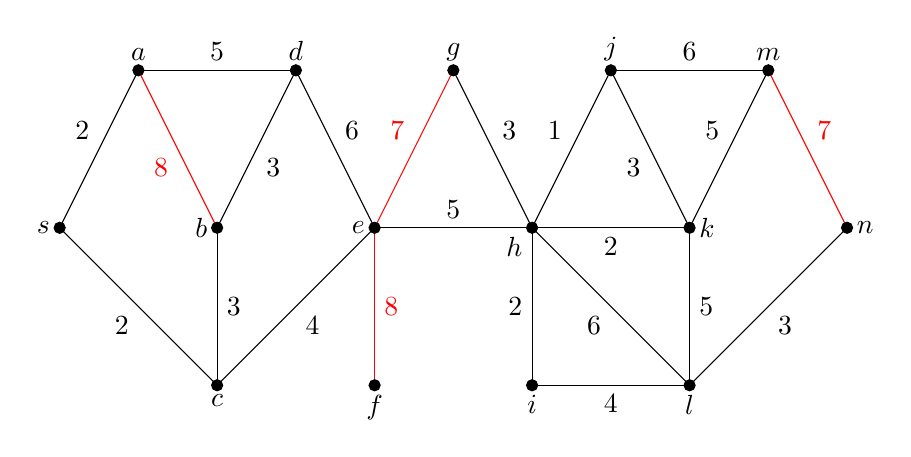
\begin{tikzpicture}

    \coordinate (a) at ( 1, 4);
\coordinate (b) at ( 2, 2);
\coordinate (c) at ( 2, 0);
\coordinate (d) at ( 3, 4);
\coordinate (e) at ( 4, 2);
\coordinate (f) at ( 4, 0);
\coordinate (g) at ( 5, 4);
\coordinate (h) at ( 6, 2);
\coordinate (i) at ( 6, 0);
\coordinate (j) at ( 7, 4);
\coordinate (k) at ( 8, 2);
\coordinate (l) at ( 8, 0);
\coordinate (m) at ( 9, 4);
\coordinate (n) at (10, 2);
\coordinate (s) at ( 0, 2);

    \draw [color = red] (a) -- node [below left]  {$8$} (b);
    \draw [color = black] (a) -- node [above]       {$5$} (d);
    \draw [color = black] (a) -- node [above left]  {$2$} (s);
    \draw [color = black] (b) -- node [right]       {$3$} (c);
    \draw [color = black] (b) -- node [below right] {$3$} (d);
    \draw [color = black] (c) -- node [below right] {$4$} (e);
    \draw [color = black] (c) -- node [below left]  {$2$} (s);
    \draw [color = black] (d) -- node [above right] {$6$} (e);
    \draw [color = red] (e) -- node [right]       {$8$} (f);
    \draw [color = red] (e) -- node [above left]  {$7$} (g);
    \draw [color = black] (e) -- node [above]       {$5$} (h);
    \draw [color = black] (g) -- node [above right] {$3$} (h);
    \draw [color = black] (h) -- node [left]        {$2$} (i);
    \draw [color = black] (h) -- node [above left]  {$1$} (j);
    \draw [color = black] (h) -- node [below]       {$2$} (k);
    \draw [color = black] (h) -- node [below left]  {$6$} (l);
    \draw [color = black] (i) -- node [below]       {$4$} (l);
    \draw [color = black] (j) -- node [below left]  {$3$} (k);
    \draw [color = black] (j) -- node [above]       {$6$} (m);
    \draw [color = black] (k) -- node [right]       {$5$} (l);
    \draw [color = black] (k) -- node [above left]  {$5$} (m);
    \draw [color = black] (l) -- node [below right] {$3$} (n);
    \draw [color = red] (m) -- node [above right] {$7$} (n);

    \filldraw [color = black] (a) circle (2pt) node [above]      {$a$};
    \filldraw [color = black] (b) circle (2pt) node [left]       {$b$};
    \filldraw [color = black] (c) circle (2pt) node [below]      {$c$};
    \filldraw [color = black] (d) circle (2pt) node [above]      {$d$};
    \filldraw [color = black] (e) circle (2pt) node [left]       {$e$};
    \filldraw [color = black] (f) circle (2pt) node [below]      {$f$};
    \filldraw [color = black] (g) circle (2pt) node [above]      {$g$};
    \filldraw [color = black] (h) circle (2pt) node [below left] {$h$};
    \filldraw [color = black] (i) circle (2pt) node [below]      {$i$};
    \filldraw [color = black] (j) circle (2pt) node [above]      {$j$};
    \filldraw [color = black] (k) circle (2pt) node [right]      {$k$};
    \filldraw [color = black] (l) circle (2pt) node [below]      {$l$};
    \filldraw [color = black] (m) circle (2pt) node [above]      {$m$};
    \filldraw [color = black] (n) circle (2pt) node [right]      {$n$};
    \filldraw [color = black]   (s) circle (2pt) node [left]       {$s$};

\end{tikzpicture}

    \end{center}

    \begin{multline*}
        P_4
        \stackrel
        {
            \Bbraces{d, e}
        }{
            \mapsto
        }
        P_5 :=
        \{
            (\Bbraces{a, b}, \Bbraces{\Bbraces{a, b}}),
            (\Bbraces{c}, \emptyset),
            (\Bbraces{d, e, f, g}, \Bbraces{\Bbraces{d, e}, \Bbraces{e, f}, \Bbraces{e, g}}), \\
            (\Bbraces{h}, \emptyset),
            (\Bbraces{i}, \emptyset),
            (\Bbraces{j}, \emptyset),
            (\Bbraces{k}, \emptyset),
            (\Bbraces{l}, \emptyset),
            (\Bbraces{m, n}, \Bbraces{\Bbraces{m, n}}),
            (\Bbraces{s}, \emptyset)
        \}
    \end{multline*}

    \begin{center}
        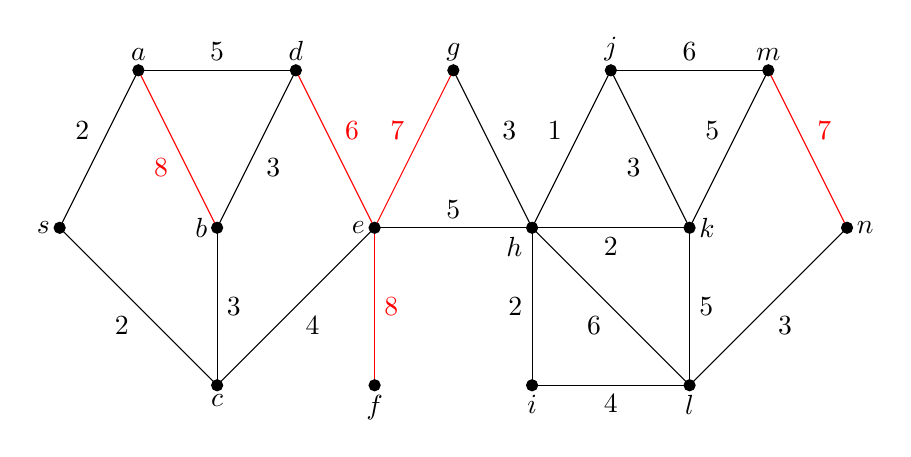
\begin{tikzpicture}

    \coordinate (a) at ( 1, 4);
\coordinate (b) at ( 2, 2);
\coordinate (c) at ( 2, 0);
\coordinate (d) at ( 3, 4);
\coordinate (e) at ( 4, 2);
\coordinate (f) at ( 4, 0);
\coordinate (g) at ( 5, 4);
\coordinate (h) at ( 6, 2);
\coordinate (i) at ( 6, 0);
\coordinate (j) at ( 7, 4);
\coordinate (k) at ( 8, 2);
\coordinate (l) at ( 8, 0);
\coordinate (m) at ( 9, 4);
\coordinate (n) at (10, 2);
\coordinate (s) at ( 0, 2);

    \draw [color = red] (a) -- node [below left]  {$8$} (b);
    \draw [color = black] (a) -- node [above]       {$5$} (d);
    \draw [color = black] (a) -- node [above left]  {$2$} (s);
    \draw [color = black] (b) -- node [right]       {$3$} (c);
    \draw [color = black] (b) -- node [below right] {$3$} (d);
    \draw [color = black] (c) -- node [below right] {$4$} (e);
    \draw [color = black] (c) -- node [below left]  {$2$} (s);
    \draw [color = red] (d) -- node [above right] {$6$} (e);
    \draw [color = red] (e) -- node [right]       {$8$} (f);
    \draw [color = red] (e) -- node [above left]  {$7$} (g);
    \draw [color = black] (e) -- node [above]       {$5$} (h);
    \draw [color = black] (g) -- node [above right] {$3$} (h);
    \draw [color = black] (h) -- node [left]        {$2$} (i);
    \draw [color = black] (h) -- node [above left]  {$1$} (j);
    \draw [color = black] (h) -- node [below]       {$2$} (k);
    \draw [color = black] (h) -- node [below left]  {$6$} (l);
    \draw [color = black] (i) -- node [below]       {$4$} (l);
    \draw [color = black] (j) -- node [below left]  {$3$} (k);
    \draw [color = black] (j) -- node [above]       {$6$} (m);
    \draw [color = black] (k) -- node [right]       {$5$} (l);
    \draw [color = black] (k) -- node [above left]  {$5$} (m);
    \draw [color = black] (l) -- node [below right] {$3$} (n);
    \draw [color = red] (m) -- node [above right] {$7$} (n);

    \filldraw [color = black] (a) circle (2pt) node [above]      {$a$};
    \filldraw [color = black] (b) circle (2pt) node [left]       {$b$};
    \filldraw [color = black] (c) circle (2pt) node [below]      {$c$};
    \filldraw [color = black] (d) circle (2pt) node [above]      {$d$};
    \filldraw [color = black] (e) circle (2pt) node [left]       {$e$};
    \filldraw [color = black] (f) circle (2pt) node [below]      {$f$};
    \filldraw [color = black] (g) circle (2pt) node [above]      {$g$};
    \filldraw [color = black] (h) circle (2pt) node [below left] {$h$};
    \filldraw [color = black] (i) circle (2pt) node [below]      {$i$};
    \filldraw [color = black] (j) circle (2pt) node [above]      {$j$};
    \filldraw [color = black] (k) circle (2pt) node [right]      {$k$};
    \filldraw [color = black] (l) circle (2pt) node [below]      {$l$};
    \filldraw [color = black] (m) circle (2pt) node [above]      {$m$};
    \filldraw [color = black] (n) circle (2pt) node [right]      {$n$};
    \filldraw [color = black]   (s) circle (2pt) node [left]       {$s$};

\end{tikzpicture}

    \end{center}

    \begin{multline*}
        P_5
        \stackrel
        {
            \Bbraces{h, l}
        }{
            \mapsto
        }
        P_6 :=
        \{
            (\Bbraces{a, b}, \Bbraces{\Bbraces{a, b}}),
            (\Bbraces{c}, \emptyset),
            (\Bbraces{d, e, f, g}, \Bbraces{\Bbraces{d, e}, \Bbraces{e, f}, \Bbraces{e, g}}), \\
            (\Bbraces{h, l}, \Bbraces{\Bbraces{h, l}}),
            (\Bbraces{i}, \emptyset),
            (\Bbraces{j}, \emptyset),
            (\Bbraces{k}, \emptyset),
            (\Bbraces{m, n}, \Bbraces{\Bbraces{m, n}}),
            (\Bbraces{s}, \emptyset)
        \}
    \end{multline*}

    \begin{center}
        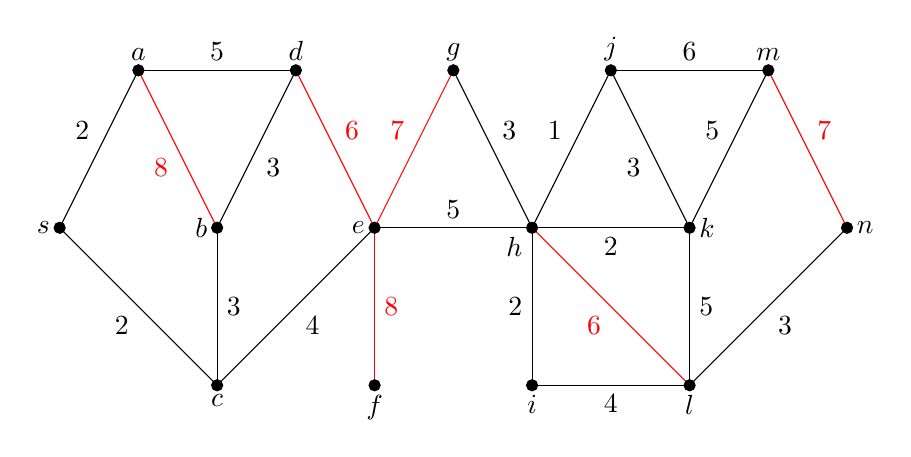
\begin{tikzpicture}

    \coordinate (a) at ( 1, 4);
\coordinate (b) at ( 2, 2);
\coordinate (c) at ( 2, 0);
\coordinate (d) at ( 3, 4);
\coordinate (e) at ( 4, 2);
\coordinate (f) at ( 4, 0);
\coordinate (g) at ( 5, 4);
\coordinate (h) at ( 6, 2);
\coordinate (i) at ( 6, 0);
\coordinate (j) at ( 7, 4);
\coordinate (k) at ( 8, 2);
\coordinate (l) at ( 8, 0);
\coordinate (m) at ( 9, 4);
\coordinate (n) at (10, 2);
\coordinate (s) at ( 0, 2);

    \draw [color = red] (a) -- node [below left]  {$8$} (b);
    \draw [color = black] (a) -- node [above]       {$5$} (d);
    \draw [color = black] (a) -- node [above left]  {$2$} (s);
    \draw [color = black] (b) -- node [right]       {$3$} (c);
    \draw [color = black] (b) -- node [below right] {$3$} (d);
    \draw [color = black] (c) -- node [below right] {$4$} (e);
    \draw [color = black] (c) -- node [below left]  {$2$} (s);
    \draw [color = red] (d) -- node [above right] {$6$} (e);
    \draw [color = red] (e) -- node [right]       {$8$} (f);
    \draw [color = red] (e) -- node [above left]  {$7$} (g);
    \draw [color = black] (e) -- node [above]       {$5$} (h);
    \draw [color = black] (g) -- node [above right] {$3$} (h);
    \draw [color = black] (h) -- node [left]        {$2$} (i);
    \draw [color = black] (h) -- node [above left]  {$1$} (j);
    \draw [color = black] (h) -- node [below]       {$2$} (k);
    \draw [color = red] (h) -- node [below left]  {$6$} (l);
    \draw [color = black] (i) -- node [below]       {$4$} (l);
    \draw [color = black] (j) -- node [below left]  {$3$} (k);
    \draw [color = black] (j) -- node [above]       {$6$} (m);
    \draw [color = black] (k) -- node [right]       {$5$} (l);
    \draw [color = black] (k) -- node [above left]  {$5$} (m);
    \draw [color = black] (l) -- node [below right] {$3$} (n);
    \draw [color = red] (m) -- node [above right] {$7$} (n);

    \filldraw [color = black] (a) circle (2pt) node [above]      {$a$};
    \filldraw [color = black] (b) circle (2pt) node [left]       {$b$};
    \filldraw [color = black] (c) circle (2pt) node [below]      {$c$};
    \filldraw [color = black] (d) circle (2pt) node [above]      {$d$};
    \filldraw [color = black] (e) circle (2pt) node [left]       {$e$};
    \filldraw [color = black] (f) circle (2pt) node [below]      {$f$};
    \filldraw [color = black] (g) circle (2pt) node [above]      {$g$};
    \filldraw [color = black] (h) circle (2pt) node [below left] {$h$};
    \filldraw [color = black] (i) circle (2pt) node [below]      {$i$};
    \filldraw [color = black] (j) circle (2pt) node [above]      {$j$};
    \filldraw [color = black] (k) circle (2pt) node [right]      {$k$};
    \filldraw [color = black] (l) circle (2pt) node [below]      {$l$};
    \filldraw [color = black] (m) circle (2pt) node [above]      {$m$};
    \filldraw [color = black] (n) circle (2pt) node [right]      {$n$};
    \filldraw [color = black]   (s) circle (2pt) node [left]       {$s$};

\end{tikzpicture}

    \end{center}

    \begin{multline*}
        P_6
        \stackrel
        {
            \Bbraces{j, m}
        }{
            \mapsto
        }
        P_7 :=
        \{
            (\Bbraces{a, b}, \Bbraces{\Bbraces{a, b}}),
            (\Bbraces{c}, \emptyset),
            (\Bbraces{d, e, f, g}, \Bbraces{\Bbraces{d, e}, \Bbraces{e, f}, \Bbraces{e, g}}), \\
            (\Bbraces{h, l}, \Bbraces{\Bbraces{h, l}}),
            (\Bbraces{i}, \emptyset),
            (\Bbraces{j, m, n}, \Bbraces{\Bbraces{j, m}, \Bbraces{m, n}}),
            (\Bbraces{k}, \emptyset),
            (\Bbraces{s}, \emptyset)
        \}
    \end{multline*}

    \begin{center}
        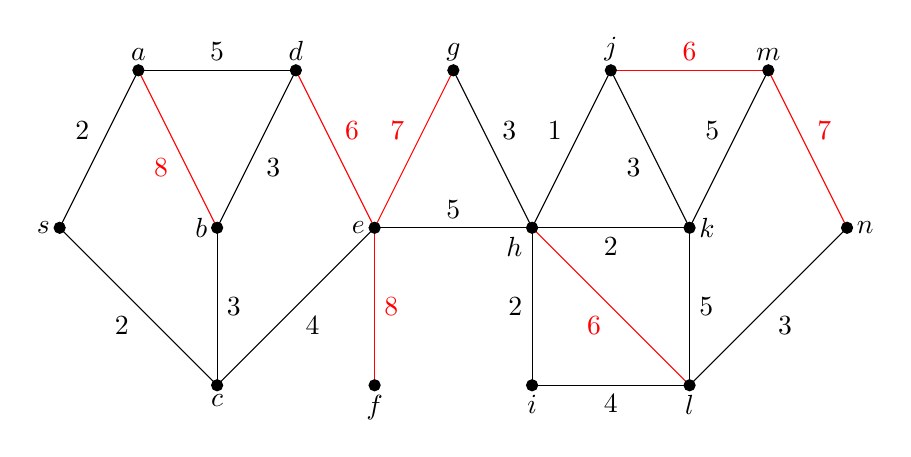
\begin{tikzpicture}

    \coordinate (a) at ( 1, 4);
\coordinate (b) at ( 2, 2);
\coordinate (c) at ( 2, 0);
\coordinate (d) at ( 3, 4);
\coordinate (e) at ( 4, 2);
\coordinate (f) at ( 4, 0);
\coordinate (g) at ( 5, 4);
\coordinate (h) at ( 6, 2);
\coordinate (i) at ( 6, 0);
\coordinate (j) at ( 7, 4);
\coordinate (k) at ( 8, 2);
\coordinate (l) at ( 8, 0);
\coordinate (m) at ( 9, 4);
\coordinate (n) at (10, 2);
\coordinate (s) at ( 0, 2);

    \draw [color = red] (a) -- node [below left]  {$8$} (b);
    \draw [color = black] (a) -- node [above]       {$5$} (d);
    \draw [color = black] (a) -- node [above left]  {$2$} (s);
    \draw [color = black] (b) -- node [right]       {$3$} (c);
    \draw [color = black] (b) -- node [below right] {$3$} (d);
    \draw [color = black] (c) -- node [below right] {$4$} (e);
    \draw [color = black] (c) -- node [below left]  {$2$} (s);
    \draw [color = red] (d) -- node [above right] {$6$} (e);
    \draw [color = red] (e) -- node [right]       {$8$} (f);
    \draw [color = red] (e) -- node [above left]  {$7$} (g);
    \draw [color = black] (e) -- node [above]       {$5$} (h);
    \draw [color = black] (g) -- node [above right] {$3$} (h);
    \draw [color = black] (h) -- node [left]        {$2$} (i);
    \draw [color = black] (h) -- node [above left]  {$1$} (j);
    \draw [color = black] (h) -- node [below]       {$2$} (k);
    \draw [color = red] (h) -- node [below left]  {$6$} (l);
    \draw [color = black] (i) -- node [below]       {$4$} (l);
    \draw [color = black] (j) -- node [below left]  {$3$} (k);
    \draw [color = red] (j) -- node [above]       {$6$} (m);
    \draw [color = black] (k) -- node [right]       {$5$} (l);
    \draw [color = black] (k) -- node [above left]  {$5$} (m);
    \draw [color = black] (l) -- node [below right] {$3$} (n);
    \draw [color = red] (m) -- node [above right] {$7$} (n);

    \filldraw [color = black] (a) circle (2pt) node [above]      {$a$};
    \filldraw [color = black] (b) circle (2pt) node [left]       {$b$};
    \filldraw [color = black] (c) circle (2pt) node [below]      {$c$};
    \filldraw [color = black] (d) circle (2pt) node [above]      {$d$};
    \filldraw [color = black] (e) circle (2pt) node [left]       {$e$};
    \filldraw [color = black] (f) circle (2pt) node [below]      {$f$};
    \filldraw [color = black] (g) circle (2pt) node [above]      {$g$};
    \filldraw [color = black] (h) circle (2pt) node [below left] {$h$};
    \filldraw [color = black] (i) circle (2pt) node [below]      {$i$};
    \filldraw [color = black] (j) circle (2pt) node [above]      {$j$};
    \filldraw [color = black] (k) circle (2pt) node [right]      {$k$};
    \filldraw [color = black] (l) circle (2pt) node [below]      {$l$};
    \filldraw [color = black] (m) circle (2pt) node [above]      {$m$};
    \filldraw [color = black] (n) circle (2pt) node [right]      {$n$};
    \filldraw [color = black]   (s) circle (2pt) node [left]       {$s$};

\end{tikzpicture}

    \end{center}

    \begin{multline*}
        P_7
        \stackrel
        {
            \Bbraces{a, d}
        }{
            \mapsto
        }
        P_8 :=
        \{
            (\Bbraces{a, b, d, e, f, g}, \Bbraces{\Bbraces{a, b}, \Bbraces{d, e}, \Bbraces{e, f}, \Bbraces{e, g}}),
            (\Bbraces{c}, \emptyset), \\
            (\Bbraces{h, l}, \Bbraces{\Bbraces{h, l}}),
            (\Bbraces{i}, \emptyset),
            (\Bbraces{j, m, n}, \Bbraces{\Bbraces{j, m}, \Bbraces{m, n}}),
            (\Bbraces{k}, \emptyset),
            (\Bbraces{s}, \emptyset)
        \}
    \end{multline*}

    \begin{center}
        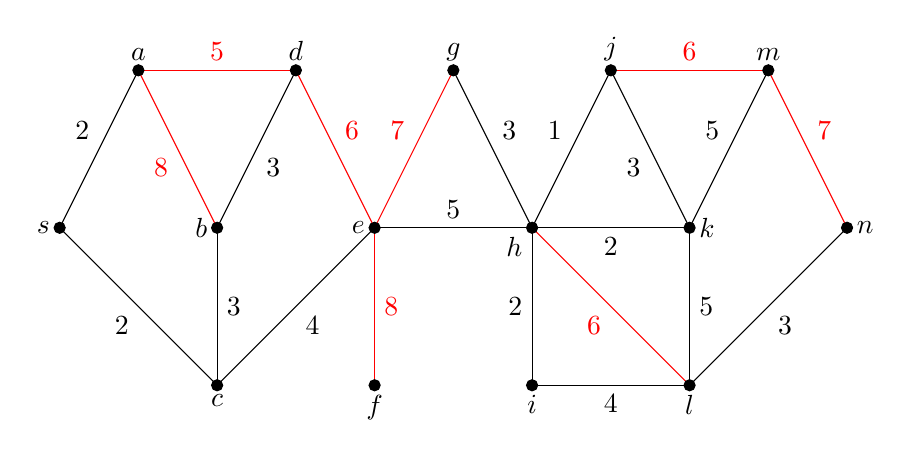
\begin{tikzpicture}

    \coordinate (a) at ( 1, 4);
\coordinate (b) at ( 2, 2);
\coordinate (c) at ( 2, 0);
\coordinate (d) at ( 3, 4);
\coordinate (e) at ( 4, 2);
\coordinate (f) at ( 4, 0);
\coordinate (g) at ( 5, 4);
\coordinate (h) at ( 6, 2);
\coordinate (i) at ( 6, 0);
\coordinate (j) at ( 7, 4);
\coordinate (k) at ( 8, 2);
\coordinate (l) at ( 8, 0);
\coordinate (m) at ( 9, 4);
\coordinate (n) at (10, 2);
\coordinate (s) at ( 0, 2);

    \draw [color = red] (a) -- node [below left]  {$8$} (b);
    \draw [color = red] (a) -- node [above]       {$5$} (d);
    \draw [color = black] (a) -- node [above left]  {$2$} (s);
    \draw [color = black] (b) -- node [right]       {$3$} (c);
    \draw [color = black] (b) -- node [below right] {$3$} (d);
    \draw [color = black] (c) -- node [below right] {$4$} (e);
    \draw [color = black] (c) -- node [below left]  {$2$} (s);
    \draw [color = red] (d) -- node [above right] {$6$} (e);
    \draw [color = red] (e) -- node [right]       {$8$} (f);
    \draw [color = red] (e) -- node [above left]  {$7$} (g);
    \draw [color = black] (e) -- node [above]       {$5$} (h);
    \draw [color = black] (g) -- node [above right] {$3$} (h);
    \draw [color = black] (h) -- node [left]        {$2$} (i);
    \draw [color = black] (h) -- node [above left]  {$1$} (j);
    \draw [color = black] (h) -- node [below]       {$2$} (k);
    \draw [color = red] (h) -- node [below left]  {$6$} (l);
    \draw [color = black] (i) -- node [below]       {$4$} (l);
    \draw [color = black] (j) -- node [below left]  {$3$} (k);
    \draw [color = red] (j) -- node [above]       {$6$} (m);
    \draw [color = black] (k) -- node [right]       {$5$} (l);
    \draw [color = black] (k) -- node [above left]  {$5$} (m);
    \draw [color = black] (l) -- node [below right] {$3$} (n);
    \draw [color = red] (m) -- node [above right] {$7$} (n);

    \filldraw [color = black] (a) circle (2pt) node [above]      {$a$};
    \filldraw [color = black] (b) circle (2pt) node [left]       {$b$};
    \filldraw [color = black] (c) circle (2pt) node [below]      {$c$};
    \filldraw [color = black] (d) circle (2pt) node [above]      {$d$};
    \filldraw [color = black] (e) circle (2pt) node [left]       {$e$};
    \filldraw [color = black] (f) circle (2pt) node [below]      {$f$};
    \filldraw [color = black] (g) circle (2pt) node [above]      {$g$};
    \filldraw [color = black] (h) circle (2pt) node [below left] {$h$};
    \filldraw [color = black] (i) circle (2pt) node [below]      {$i$};
    \filldraw [color = black] (j) circle (2pt) node [above]      {$j$};
    \filldraw [color = black] (k) circle (2pt) node [right]      {$k$};
    \filldraw [color = black] (l) circle (2pt) node [below]      {$l$};
    \filldraw [color = black] (m) circle (2pt) node [above]      {$m$};
    \filldraw [color = black] (n) circle (2pt) node [right]      {$n$};
    \filldraw [color = black]   (s) circle (2pt) node [left]       {$s$};

\end{tikzpicture}

    \end{center}

    \begin{multline*}
        P_8
        \stackrel
        {
            \Bbraces{e, h}
        }{
            \mapsto
        }
        P_9 :=
        \{
            (\Bbraces{a, b, d, e, f, g, h, l}, \Bbraces{\Bbraces{a, b}, \Bbraces{d, e}, \Bbraces{e, f}, \Bbraces{e, g}, \Bbraces{h, l}}),
            (\Bbraces{c}, \emptyset), \\
            (\Bbraces{i}, \emptyset),
            (\Bbraces{j, m, n}, \Bbraces{\Bbraces{j, m}, \Bbraces{m, n}}),
            (\Bbraces{k}, \emptyset),
            (\Bbraces{s}, \emptyset)
        \}
    \end{multline*}

    \begin{center}
        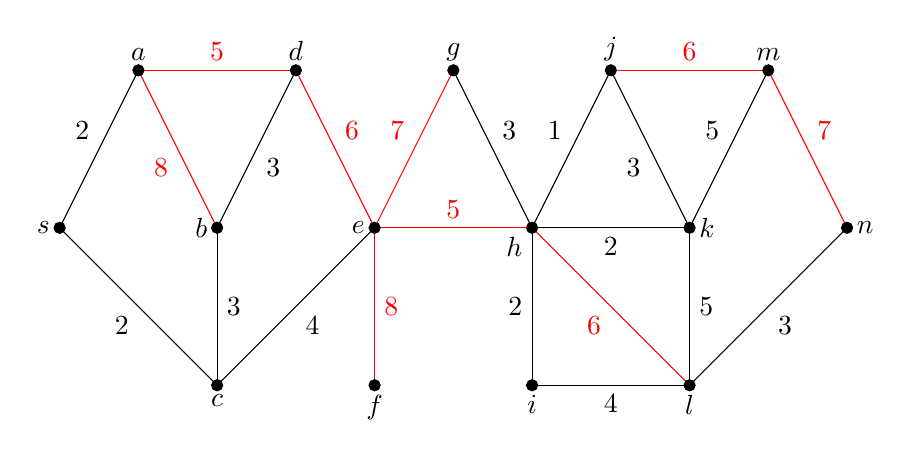
\begin{tikzpicture}

    \coordinate (a) at ( 1, 4);
\coordinate (b) at ( 2, 2);
\coordinate (c) at ( 2, 0);
\coordinate (d) at ( 3, 4);
\coordinate (e) at ( 4, 2);
\coordinate (f) at ( 4, 0);
\coordinate (g) at ( 5, 4);
\coordinate (h) at ( 6, 2);
\coordinate (i) at ( 6, 0);
\coordinate (j) at ( 7, 4);
\coordinate (k) at ( 8, 2);
\coordinate (l) at ( 8, 0);
\coordinate (m) at ( 9, 4);
\coordinate (n) at (10, 2);
\coordinate (s) at ( 0, 2);

    \draw [color = red] (a) -- node [below left]  {$8$} (b);
    \draw [color = red] (a) -- node [above]       {$5$} (d);
    \draw [color = black] (a) -- node [above left]  {$2$} (s);
    \draw [color = black] (b) -- node [right]       {$3$} (c);
    \draw [color = black] (b) -- node [below right] {$3$} (d);
    \draw [color = black] (c) -- node [below right] {$4$} (e);
    \draw [color = black] (c) -- node [below left]  {$2$} (s);
    \draw [color = red] (d) -- node [above right] {$6$} (e);
    \draw [color = red] (e) -- node [right]       {$8$} (f);
    \draw [color = red] (e) -- node [above left]  {$7$} (g);
    \draw [color = red] (e) -- node [above]       {$5$} (h);
    \draw [color = black] (g) -- node [above right] {$3$} (h);
    \draw [color = black] (h) -- node [left]        {$2$} (i);
    \draw [color = black] (h) -- node [above left]  {$1$} (j);
    \draw [color = black] (h) -- node [below]       {$2$} (k);
    \draw [color = red] (h) -- node [below left]  {$6$} (l);
    \draw [color = black] (i) -- node [below]       {$4$} (l);
    \draw [color = black] (j) -- node [below left]  {$3$} (k);
    \draw [color = red] (j) -- node [above]       {$6$} (m);
    \draw [color = black] (k) -- node [right]       {$5$} (l);
    \draw [color = black] (k) -- node [above left]  {$5$} (m);
    \draw [color = black] (l) -- node [below right] {$3$} (n);
    \draw [color = red] (m) -- node [above right] {$7$} (n);

    \filldraw [color = black] (a) circle (2pt) node [above]      {$a$};
    \filldraw [color = black] (b) circle (2pt) node [left]       {$b$};
    \filldraw [color = black] (c) circle (2pt) node [below]      {$c$};
    \filldraw [color = black] (d) circle (2pt) node [above]      {$d$};
    \filldraw [color = black] (e) circle (2pt) node [left]       {$e$};
    \filldraw [color = black] (f) circle (2pt) node [below]      {$f$};
    \filldraw [color = black] (g) circle (2pt) node [above]      {$g$};
    \filldraw [color = black] (h) circle (2pt) node [below left] {$h$};
    \filldraw [color = black] (i) circle (2pt) node [below]      {$i$};
    \filldraw [color = black] (j) circle (2pt) node [above]      {$j$};
    \filldraw [color = black] (k) circle (2pt) node [right]      {$k$};
    \filldraw [color = black] (l) circle (2pt) node [below]      {$l$};
    \filldraw [color = black] (m) circle (2pt) node [above]      {$m$};
    \filldraw [color = black] (n) circle (2pt) node [right]      {$n$};
    \filldraw [color = black]   (s) circle (2pt) node [left]       {$s$};

\end{tikzpicture}

    \end{center}

    \begin{multline*}
        P_9
        \stackrel
        {
            \Bbraces{k, l}
        }{
            \mapsto
        }
        P_{10} :=
        \{
            (\Bbraces{a, b, d, e, f, g, h, k, l}, \Bbraces{\Bbraces{a, b}, \Bbraces{d, e}, \Bbraces{e, f}, \Bbraces{e, g}, \Bbraces{h, l}, \Bbraces{k, l}}),
            (\Bbraces{c}, \emptyset), \\
            (\Bbraces{i}, \emptyset),
            (\Bbraces{j, m, n}, \Bbraces{\Bbraces{j, m}, \Bbraces{m, n}}),
            (\Bbraces{s}, \emptyset)
        \}
    \end{multline*}

    \begin{center}
        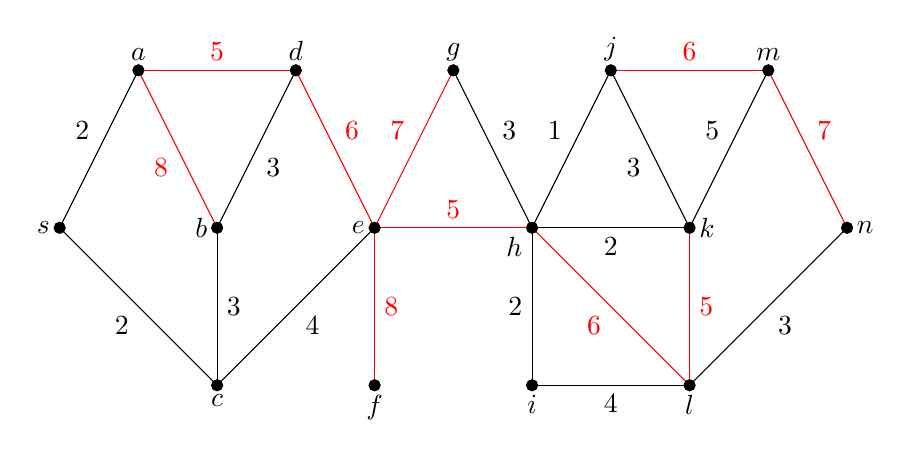
\begin{tikzpicture}

    \coordinate (a) at ( 1, 4);
\coordinate (b) at ( 2, 2);
\coordinate (c) at ( 2, 0);
\coordinate (d) at ( 3, 4);
\coordinate (e) at ( 4, 2);
\coordinate (f) at ( 4, 0);
\coordinate (g) at ( 5, 4);
\coordinate (h) at ( 6, 2);
\coordinate (i) at ( 6, 0);
\coordinate (j) at ( 7, 4);
\coordinate (k) at ( 8, 2);
\coordinate (l) at ( 8, 0);
\coordinate (m) at ( 9, 4);
\coordinate (n) at (10, 2);
\coordinate (s) at ( 0, 2);

    \draw [color = red] (a) -- node [below left]  {$8$} (b);
    \draw [color = red] (a) -- node [above]       {$5$} (d);
    \draw [color = black] (a) -- node [above left]  {$2$} (s);
    \draw [color = black] (b) -- node [right]       {$3$} (c);
    \draw [color = black] (b) -- node [below right] {$3$} (d);
    \draw [color = black] (c) -- node [below right] {$4$} (e);
    \draw [color = black] (c) -- node [below left]  {$2$} (s);
    \draw [color = red] (d) -- node [above right] {$6$} (e);
    \draw [color = red] (e) -- node [right]       {$8$} (f);
    \draw [color = red] (e) -- node [above left]  {$7$} (g);
    \draw [color = red] (e) -- node [above]       {$5$} (h);
    \draw [color = black] (g) -- node [above right] {$3$} (h);
    \draw [color = black] (h) -- node [left]        {$2$} (i);
    \draw [color = black] (h) -- node [above left]  {$1$} (j);
    \draw [color = black] (h) -- node [below]       {$2$} (k);
    \draw [color = red] (h) -- node [below left]  {$6$} (l);
    \draw [color = black] (i) -- node [below]       {$4$} (l);
    \draw [color = black] (j) -- node [below left]  {$3$} (k);
    \draw [color = red] (j) -- node [above]       {$6$} (m);
    \draw [color = red] (k) -- node [right]       {$5$} (l);
    \draw [color = black] (k) -- node [above left]  {$5$} (m);
    \draw [color = black] (l) -- node [below right] {$3$} (n);
    \draw [color = red] (m) -- node [above right] {$7$} (n);

    \filldraw [color = black] (a) circle (2pt) node [above]      {$a$};
    \filldraw [color = black] (b) circle (2pt) node [left]       {$b$};
    \filldraw [color = black] (c) circle (2pt) node [below]      {$c$};
    \filldraw [color = black] (d) circle (2pt) node [above]      {$d$};
    \filldraw [color = black] (e) circle (2pt) node [left]       {$e$};
    \filldraw [color = black] (f) circle (2pt) node [below]      {$f$};
    \filldraw [color = black] (g) circle (2pt) node [above]      {$g$};
    \filldraw [color = black] (h) circle (2pt) node [below left] {$h$};
    \filldraw [color = black] (i) circle (2pt) node [below]      {$i$};
    \filldraw [color = black] (j) circle (2pt) node [above]      {$j$};
    \filldraw [color = black] (k) circle (2pt) node [right]      {$k$};
    \filldraw [color = black] (l) circle (2pt) node [below]      {$l$};
    \filldraw [color = black] (m) circle (2pt) node [above]      {$m$};
    \filldraw [color = black] (n) circle (2pt) node [right]      {$n$};
    \filldraw [color = black]   (s) circle (2pt) node [left]       {$s$};

\end{tikzpicture}

    \end{center}

    \begin{multline*}
        P_{10}
        \stackrel
        {
            \Bbraces{k, m}
        }{
            \mapsto
        }
        P_{11} :=
        \{
            (\Bbraces{a, b, d, e, f, g, h, j, k, l, m, n}, \\ \Bbraces{\Bbraces{a, b}, \Bbraces{d, e}, \Bbraces{e, f}, \Bbraces{e, g}, \Bbraces{h, l}, \Bbraces{j, m}, \Bbraces{k, l}, \Bbraces{m, n}}),
            (\Bbraces{c}, \emptyset),
            (\Bbraces{i}, \emptyset),
            (\Bbraces{s}, \emptyset)
        \}
    \end{multline*}

    \begin{center}
        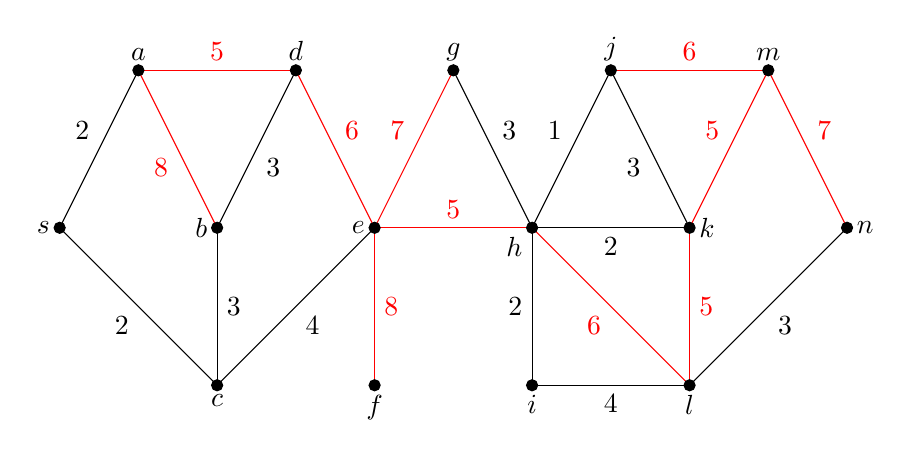
\begin{tikzpicture}

    \coordinate (a) at ( 1, 4);
\coordinate (b) at ( 2, 2);
\coordinate (c) at ( 2, 0);
\coordinate (d) at ( 3, 4);
\coordinate (e) at ( 4, 2);
\coordinate (f) at ( 4, 0);
\coordinate (g) at ( 5, 4);
\coordinate (h) at ( 6, 2);
\coordinate (i) at ( 6, 0);
\coordinate (j) at ( 7, 4);
\coordinate (k) at ( 8, 2);
\coordinate (l) at ( 8, 0);
\coordinate (m) at ( 9, 4);
\coordinate (n) at (10, 2);
\coordinate (s) at ( 0, 2);

    \draw [color = red] (a) -- node [below left]  {$8$} (b);
    \draw [color = red] (a) -- node [above]       {$5$} (d);
    \draw [color = black] (a) -- node [above left]  {$2$} (s);
    \draw [color = black] (b) -- node [right]       {$3$} (c);
    \draw [color = black] (b) -- node [below right] {$3$} (d);
    \draw [color = black] (c) -- node [below right] {$4$} (e);
    \draw [color = black] (c) -- node [below left]  {$2$} (s);
    \draw [color = red] (d) -- node [above right] {$6$} (e);
    \draw [color = red] (e) -- node [right]       {$8$} (f);
    \draw [color = red] (e) -- node [above left]  {$7$} (g);
    \draw [color = red] (e) -- node [above]       {$5$} (h);
    \draw [color = black] (g) -- node [above right] {$3$} (h);
    \draw [color = black] (h) -- node [left]        {$2$} (i);
    \draw [color = black] (h) -- node [above left]  {$1$} (j);
    \draw [color = black] (h) -- node [below]       {$2$} (k);
    \draw [color = red] (h) -- node [below left]  {$6$} (l);
    \draw [color = black] (i) -- node [below]       {$4$} (l);
    \draw [color = black] (j) -- node [below left]  {$3$} (k);
    \draw [color = red] (j) -- node [above]       {$6$} (m);
    \draw [color = red] (k) -- node [right]       {$5$} (l);
    \draw [color = red] (k) -- node [above left]  {$5$} (m);
    \draw [color = black] (l) -- node [below right] {$3$} (n);
    \draw [color = red] (m) -- node [above right] {$7$} (n);

    \filldraw [color = black] (a) circle (2pt) node [above]      {$a$};
    \filldraw [color = black] (b) circle (2pt) node [left]       {$b$};
    \filldraw [color = black] (c) circle (2pt) node [below]      {$c$};
    \filldraw [color = black] (d) circle (2pt) node [above]      {$d$};
    \filldraw [color = black] (e) circle (2pt) node [left]       {$e$};
    \filldraw [color = black] (f) circle (2pt) node [below]      {$f$};
    \filldraw [color = black] (g) circle (2pt) node [above]      {$g$};
    \filldraw [color = black] (h) circle (2pt) node [below left] {$h$};
    \filldraw [color = black] (i) circle (2pt) node [below]      {$i$};
    \filldraw [color = black] (j) circle (2pt) node [above]      {$j$};
    \filldraw [color = black] (k) circle (2pt) node [right]      {$k$};
    \filldraw [color = black] (l) circle (2pt) node [below]      {$l$};
    \filldraw [color = black] (m) circle (2pt) node [above]      {$m$};
    \filldraw [color = black] (n) circle (2pt) node [right]      {$n$};
    \filldraw [color = black]   (s) circle (2pt) node [left]       {$s$};

\end{tikzpicture}

    \end{center}

    \begin{multline*}
        P_{11}
        \stackrel
        {
            \Bbraces{c, e}
        }{
            \mapsto
        }
        P_{12} :=
        \{
            (\Bbraces{a, b, c, d, e, f, g, h, j, k, l, m, n}, \\ \Bbraces{\Bbraces{a, b}, \Bbraces{c, e}, \Bbraces{d, e}, \Bbraces{e, f}, \Bbraces{e, g}, \Bbraces{h, l}, \Bbraces{j, m}, \Bbraces{k, l}, \Bbraces{m, n}}),
            (\Bbraces{i}, \emptyset),
            (\Bbraces{s}, \emptyset)
        \}
    \end{multline*}

    \begin{center}
        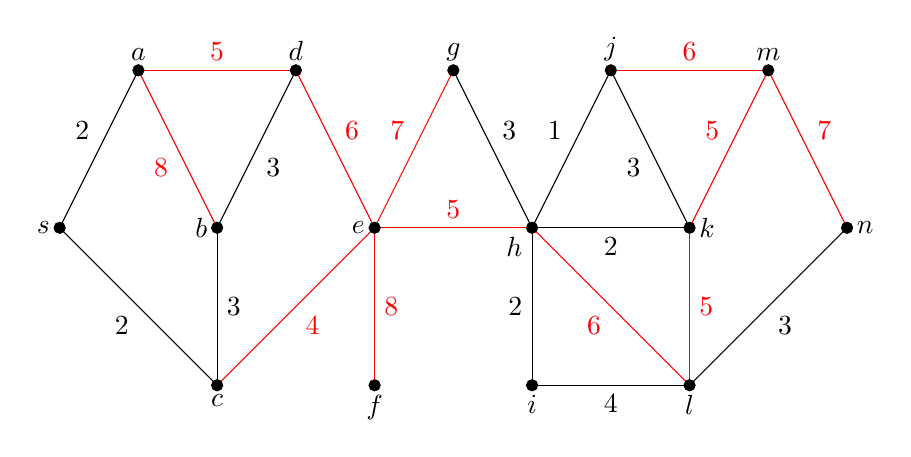
\begin{tikzpicture}

    \coordinate (a) at ( 1, 4);
\coordinate (b) at ( 2, 2);
\coordinate (c) at ( 2, 0);
\coordinate (d) at ( 3, 4);
\coordinate (e) at ( 4, 2);
\coordinate (f) at ( 4, 0);
\coordinate (g) at ( 5, 4);
\coordinate (h) at ( 6, 2);
\coordinate (i) at ( 6, 0);
\coordinate (j) at ( 7, 4);
\coordinate (k) at ( 8, 2);
\coordinate (l) at ( 8, 0);
\coordinate (m) at ( 9, 4);
\coordinate (n) at (10, 2);
\coordinate (s) at ( 0, 2);

    \draw [color = red] (a) -- node [below left]  {$8$} (b);
    \draw [color = red] (a) -- node [above]       {$5$} (d);
    \draw [color = black] (a) -- node [above left]  {$2$} (s);
    \draw [color = black] (b) -- node [right]       {$3$} (c);
    \draw [color = black] (b) -- node [below right] {$3$} (d);
    \draw [color = red] (c) -- node [below right] {$4$} (e);
    \draw [color = black] (c) -- node [below left]  {$2$} (s);
    \draw [color = red] (d) -- node [above right] {$6$} (e);
    \draw [color = red] (e) -- node [right]       {$8$} (f);
    \draw [color = red] (e) -- node [above left]  {$7$} (g);
    \draw [color = red] (e) -- node [above]       {$5$} (h);
    \draw [color = black] (g) -- node [above right] {$3$} (h);
    \draw [color = black] (h) -- node [left]        {$2$} (i);
    \draw [color = black] (h) -- node [above left]  {$1$} (j);
    \draw [color = black] (h) -- node [below]       {$2$} (k);
    \draw [color = red] (h) -- node [below left]  {$6$} (l);
    \draw [color = black] (i) -- node [below]       {$4$} (l);
    \draw [color = black] (j) -- node [below left]  {$3$} (k);
    \draw [color = red] (j) -- node [above]       {$6$} (m);
    \draw [color = red] (k) -- node [right]       {$5$} (l);
    \draw [color = red] (k) -- node [above left]  {$5$} (m);
    \draw [color = black] (l) -- node [below right] {$3$} (n);
    \draw [color = red] (m) -- node [above right] {$7$} (n);

    \filldraw [color = black] (a) circle (2pt) node [above]      {$a$};
    \filldraw [color = black] (b) circle (2pt) node [left]       {$b$};
    \filldraw [color = black] (c) circle (2pt) node [below]      {$c$};
    \filldraw [color = black] (d) circle (2pt) node [above]      {$d$};
    \filldraw [color = black] (e) circle (2pt) node [left]       {$e$};
    \filldraw [color = black] (f) circle (2pt) node [below]      {$f$};
    \filldraw [color = black] (g) circle (2pt) node [above]      {$g$};
    \filldraw [color = black] (h) circle (2pt) node [below left] {$h$};
    \filldraw [color = black] (i) circle (2pt) node [below]      {$i$};
    \filldraw [color = black] (j) circle (2pt) node [above]      {$j$};
    \filldraw [color = black] (k) circle (2pt) node [right]      {$k$};
    \filldraw [color = black] (l) circle (2pt) node [below]      {$l$};
    \filldraw [color = black] (m) circle (2pt) node [above]      {$m$};
    \filldraw [color = black] (n) circle (2pt) node [right]      {$n$};
    \filldraw [color = black]   (s) circle (2pt) node [left]       {$s$};

\end{tikzpicture}

    \end{center}

    \begin{multline*}
        P_{12}
        \stackrel
        {
            \Bbraces{i, l}
        }{
            \mapsto
        }
        P_{13} :=
        \{
            (\Bbraces{a, b, c, d, e, f, g, h, i, j, k, l, m, n}, \\ \Bbraces{\Bbraces{a, b}, \Bbraces{c, e}, \Bbraces{d, e}, \Bbraces{e, f}, \Bbraces{e, g}, \Bbraces{h, l}, \Bbraces{i, l} \Bbraces{j, m}, \Bbraces{k, l}, \Bbraces{m, n}}),
            (\Bbraces{s}, \emptyset)
        \}
    \end{multline*}

    \begin{center}
        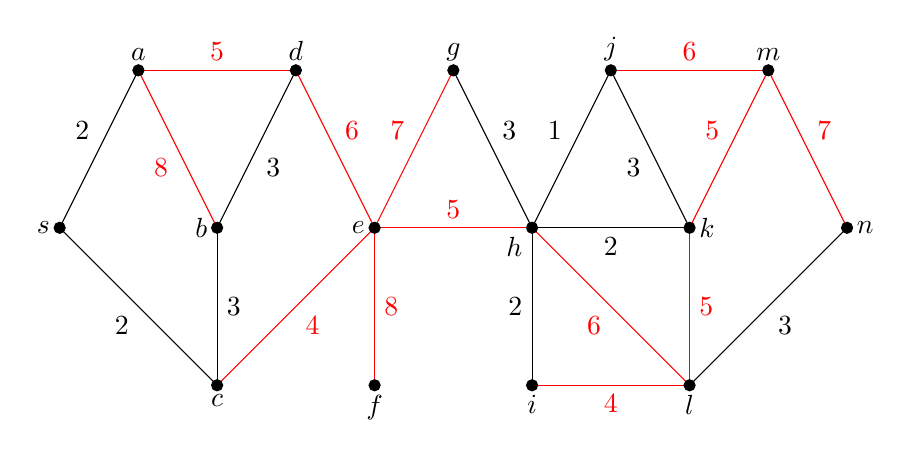
\begin{tikzpicture}

    \coordinate (a) at ( 1, 4);
\coordinate (b) at ( 2, 2);
\coordinate (c) at ( 2, 0);
\coordinate (d) at ( 3, 4);
\coordinate (e) at ( 4, 2);
\coordinate (f) at ( 4, 0);
\coordinate (g) at ( 5, 4);
\coordinate (h) at ( 6, 2);
\coordinate (i) at ( 6, 0);
\coordinate (j) at ( 7, 4);
\coordinate (k) at ( 8, 2);
\coordinate (l) at ( 8, 0);
\coordinate (m) at ( 9, 4);
\coordinate (n) at (10, 2);
\coordinate (s) at ( 0, 2);

    \draw [color = red] (a) -- node [below left]  {$8$} (b);
    \draw [color = red] (a) -- node [above]       {$5$} (d);
    \draw [color = black] (a) -- node [above left]  {$2$} (s);
    \draw [color = black] (b) -- node [right]       {$3$} (c);
    \draw [color = black] (b) -- node [below right] {$3$} (d);
    \draw [color = red] (c) -- node [below right] {$4$} (e);
    \draw [color = black] (c) -- node [below left]  {$2$} (s);
    \draw [color = red] (d) -- node [above right] {$6$} (e);
    \draw [color = red] (e) -- node [right]       {$8$} (f);
    \draw [color = red] (e) -- node [above left]  {$7$} (g);
    \draw [color = red] (e) -- node [above]       {$5$} (h);
    \draw [color = black] (g) -- node [above right] {$3$} (h);
    \draw [color = black] (h) -- node [left]        {$2$} (i);
    \draw [color = black] (h) -- node [above left]  {$1$} (j);
    \draw [color = black] (h) -- node [below]       {$2$} (k);
    \draw [color = red] (h) -- node [below left]  {$6$} (l);
    \draw [color = red] (i) -- node [below]       {$4$} (l);
    \draw [color = black] (j) -- node [below left]  {$3$} (k);
    \draw [color = red] (j) -- node [above]       {$6$} (m);
    \draw [color = red] (k) -- node [right]       {$5$} (l);
    \draw [color = red] (k) -- node [above left]  {$5$} (m);
    \draw [color = black] (l) -- node [below right] {$3$} (n);
    \draw [color = red] (m) -- node [above right] {$7$} (n);

    \filldraw [color = black] (a) circle (2pt) node [above]      {$a$};
    \filldraw [color = black] (b) circle (2pt) node [left]       {$b$};
    \filldraw [color = black] (c) circle (2pt) node [below]      {$c$};
    \filldraw [color = black] (d) circle (2pt) node [above]      {$d$};
    \filldraw [color = black] (e) circle (2pt) node [left]       {$e$};
    \filldraw [color = black] (f) circle (2pt) node [below]      {$f$};
    \filldraw [color = black] (g) circle (2pt) node [above]      {$g$};
    \filldraw [color = black] (h) circle (2pt) node [below left] {$h$};
    \filldraw [color = black] (i) circle (2pt) node [below]      {$i$};
    \filldraw [color = black] (j) circle (2pt) node [above]      {$j$};
    \filldraw [color = black] (k) circle (2pt) node [right]      {$k$};
    \filldraw [color = black] (l) circle (2pt) node [below]      {$l$};
    \filldraw [color = black] (m) circle (2pt) node [above]      {$m$};
    \filldraw [color = black] (n) circle (2pt) node [right]      {$n$};
    \filldraw [color = black]   (s) circle (2pt) node [left]       {$s$};

\end{tikzpicture}

    \end{center}

    \begin{align*}
        P_{13}
        \stackrel
        {
            \Bbraces{b, c}
        }{
            \mapsto
        }
        P_{14} := P_{13}
    \end{align*}

    \begin{align*}
        \dots
    \end{align*}

    \begin{center}
        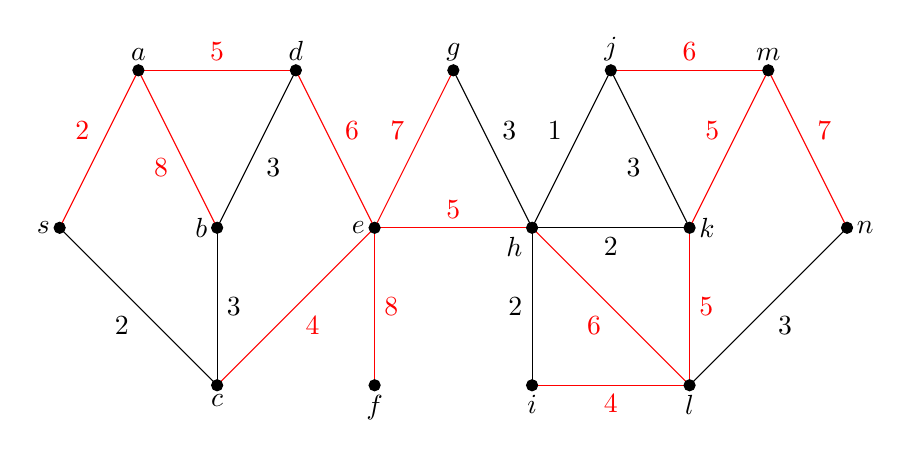
\begin{tikzpicture}

    \coordinate (a) at ( 1, 4);
\coordinate (b) at ( 2, 2);
\coordinate (c) at ( 2, 0);
\coordinate (d) at ( 3, 4);
\coordinate (e) at ( 4, 2);
\coordinate (f) at ( 4, 0);
\coordinate (g) at ( 5, 4);
\coordinate (h) at ( 6, 2);
\coordinate (i) at ( 6, 0);
\coordinate (j) at ( 7, 4);
\coordinate (k) at ( 8, 2);
\coordinate (l) at ( 8, 0);
\coordinate (m) at ( 9, 4);
\coordinate (n) at (10, 2);
\coordinate (s) at ( 0, 2);

    \draw [color = red] (a) -- node [below left]  {$8$} (b);
    \draw [color = red] (a) -- node [above]       {$5$} (d);
    \draw [color = red] (a) -- node [above left]  {$2$} (s);
    \draw [color = black] (b) -- node [right]       {$3$} (c);
    \draw [color = black] (b) -- node [below right] {$3$} (d);
    \draw [color = red] (c) -- node [below right] {$4$} (e);
    \draw [color = black] (c) -- node [below left]  {$2$} (s);
    \draw [color = red] (d) -- node [above right] {$6$} (e);
    \draw [color = red] (e) -- node [right]       {$8$} (f);
    \draw [color = red] (e) -- node [above left]  {$7$} (g);
    \draw [color = red] (e) -- node [above]       {$5$} (h);
    \draw [color = black] (g) -- node [above right] {$3$} (h);
    \draw [color = black] (h) -- node [left]        {$2$} (i);
    \draw [color = black] (h) -- node [above left]  {$1$} (j);
    \draw [color = black] (h) -- node [below]       {$2$} (k);
    \draw [color = red] (h) -- node [below left]  {$6$} (l);
    \draw [color = red] (i) -- node [below]       {$4$} (l);
    \draw [color = black] (j) -- node [below left]  {$3$} (k);
    \draw [color = red] (j) -- node [above]       {$6$} (m);
    \draw [color = red] (k) -- node [right]       {$5$} (l);
    \draw [color = red] (k) -- node [above left]  {$5$} (m);
    \draw [color = black] (l) -- node [below right] {$3$} (n);
    \draw [color = red] (m) -- node [above right] {$7$} (n);

    \filldraw [color = black] (a) circle (2pt) node [above]      {$a$};
    \filldraw [color = black] (b) circle (2pt) node [left]       {$b$};
    \filldraw [color = black] (c) circle (2pt) node [below]      {$c$};
    \filldraw [color = black] (d) circle (2pt) node [above]      {$d$};
    \filldraw [color = black] (e) circle (2pt) node [left]       {$e$};
    \filldraw [color = black] (f) circle (2pt) node [below]      {$f$};
    \filldraw [color = black] (g) circle (2pt) node [above]      {$g$};
    \filldraw [color = black] (h) circle (2pt) node [below left] {$h$};
    \filldraw [color = black] (i) circle (2pt) node [below]      {$i$};
    \filldraw [color = black] (j) circle (2pt) node [above]      {$j$};
    \filldraw [color = black] (k) circle (2pt) node [right]      {$k$};
    \filldraw [color = black] (l) circle (2pt) node [below]      {$l$};
    \filldraw [color = black] (m) circle (2pt) node [above]      {$m$};
    \filldraw [color = black] (n) circle (2pt) node [right]      {$n$};
    \filldraw [color = black]   (s) circle (2pt) node [left]       {$s$};

\end{tikzpicture}

    \end{center}

    Nachdem $G$ als zusammenhängend vorausgesetzt war, werden alle ursprünglichen Äquivalenzklassen (d.h. $1$-punktige Bäume) durch eine Kante getroffen.

    \item Algorithmus (von Prim):

    \includegraphicsboxed{DGA/DGA - Definition 7.1.png}
    \includegraphicsboxed{DGA/DGA - Algorithmus von Prim.png}

    \begin{center}
        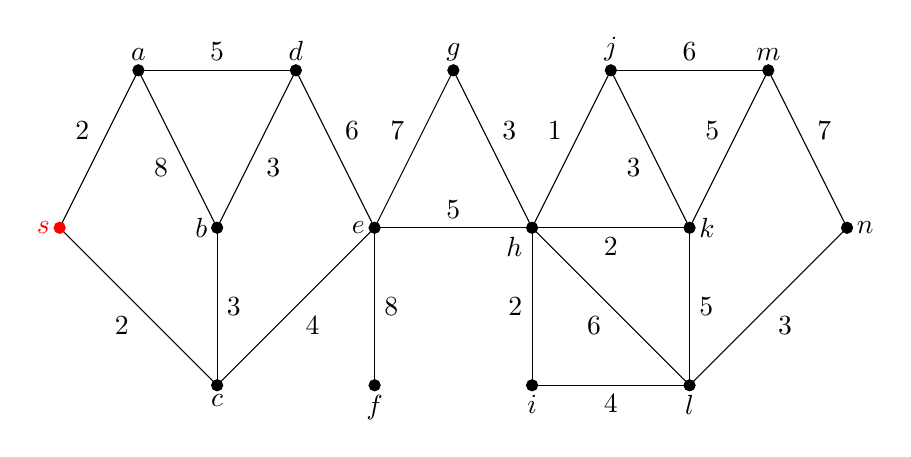
\begin{tikzpicture}

    \coordinate (a) at ( 1, 4);
\coordinate (b) at ( 2, 2);
\coordinate (c) at ( 2, 0);
\coordinate (d) at ( 3, 4);
\coordinate (e) at ( 4, 2);
\coordinate (f) at ( 4, 0);
\coordinate (g) at ( 5, 4);
\coordinate (h) at ( 6, 2);
\coordinate (i) at ( 6, 0);
\coordinate (j) at ( 7, 4);
\coordinate (k) at ( 8, 2);
\coordinate (l) at ( 8, 0);
\coordinate (m) at ( 9, 4);
\coordinate (n) at (10, 2);
\coordinate (s) at ( 0, 2);

    \draw [color = black] (a) -- node [below left]  {$8$} (b);
    \draw [color = black] (a) -- node [above]       {$5$} (d);
    \draw [color = black] (a) -- node [above left]  {$2$} (s);
    \draw [color = black] (b) -- node [right]       {$3$} (c);
    \draw [color = black] (b) -- node [below right] {$3$} (d);
    \draw [color = black] (c) -- node [below right] {$4$} (e);
    \draw [color = black] (c) -- node [below left]  {$2$} (s);
    \draw [color = black] (d) -- node [above right] {$6$} (e);
    \draw [color = black] (e) -- node [right]       {$8$} (f);
    \draw [color = black] (e) -- node [above left]  {$7$} (g);
    \draw [color = black] (e) -- node [above]       {$5$} (h);
    \draw [color = black] (g) -- node [above right] {$3$} (h);
    \draw [color = black] (h) -- node [left]        {$2$} (i);
    \draw [color = black] (h) -- node [above left]  {$1$} (j);
    \draw [color = black] (h) -- node [below]       {$2$} (k);
    \draw [color = black] (h) -- node [below left]  {$6$} (l);
    \draw [color = black] (i) -- node [below]       {$4$} (l);
    \draw [color = black] (j) -- node [below left]  {$3$} (k);
    \draw [color = black] (j) -- node [above]       {$6$} (m);
    \draw [color = black] (k) -- node [right]       {$5$} (l);
    \draw [color = black] (k) -- node [above left]  {$5$} (m);
    \draw [color = black] (l) -- node [below right] {$3$} (n);
    \draw [color = black] (m) -- node [above right] {$7$} (n);

    \filldraw [color = black] (a) circle (2pt) node [above]      {$a$};
    \filldraw [color = black] (b) circle (2pt) node [left]       {$b$};
    \filldraw [color = black] (c) circle (2pt) node [below]      {$c$};
    \filldraw [color = black] (d) circle (2pt) node [above]      {$d$};
    \filldraw [color = black] (e) circle (2pt) node [left]       {$e$};
    \filldraw [color = black] (f) circle (2pt) node [below]      {$f$};
    \filldraw [color = black] (g) circle (2pt) node [above]      {$g$};
    \filldraw [color = black] (h) circle (2pt) node [below left] {$h$};
    \filldraw [color = black] (i) circle (2pt) node [below]      {$i$};
    \filldraw [color = black] (j) circle (2pt) node [above]      {$j$};
    \filldraw [color = black] (k) circle (2pt) node [right]      {$k$};
    \filldraw [color = black] (l) circle (2pt) node [below]      {$l$};
    \filldraw [color = black] (m) circle (2pt) node [above]      {$m$};
    \filldraw [color = black] (n) circle (2pt) node [right]      {$n$};
    \filldraw [color = red]   (s) circle (2pt) node [left]       {$s$};

\end{tikzpicture}

    \end{center}

    \begin{center}
        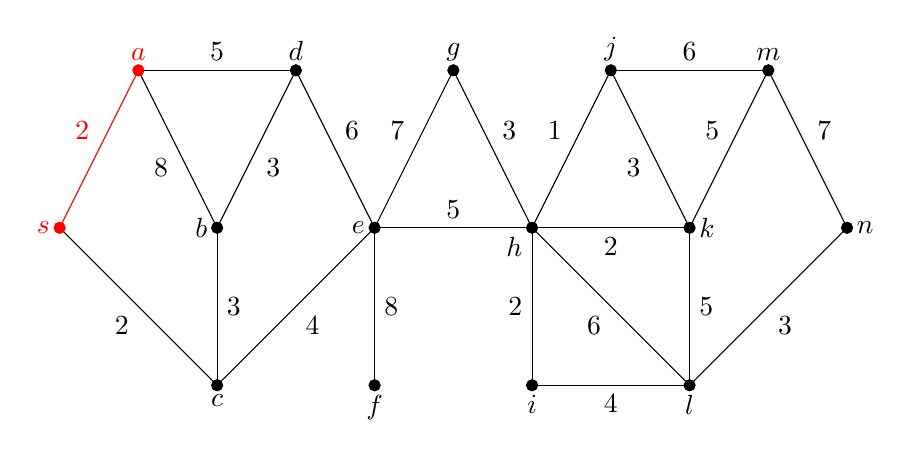
\begin{tikzpicture}

    \coordinate (a) at ( 1, 4);
\coordinate (b) at ( 2, 2);
\coordinate (c) at ( 2, 0);
\coordinate (d) at ( 3, 4);
\coordinate (e) at ( 4, 2);
\coordinate (f) at ( 4, 0);
\coordinate (g) at ( 5, 4);
\coordinate (h) at ( 6, 2);
\coordinate (i) at ( 6, 0);
\coordinate (j) at ( 7, 4);
\coordinate (k) at ( 8, 2);
\coordinate (l) at ( 8, 0);
\coordinate (m) at ( 9, 4);
\coordinate (n) at (10, 2);
\coordinate (s) at ( 0, 2);

    \draw [color = black] (a) -- node [below left]  {$8$} (b);
    \draw [color = black] (a) -- node [above]       {$5$} (d);
    \draw [color = red]   (a) -- node [above left]  {$2$} (s);
    \draw [color = black] (b) -- node [right]       {$3$} (c);
    \draw [color = black] (b) -- node [below right] {$3$} (d);
    \draw [color = black] (c) -- node [below right] {$4$} (e);
    \draw [color = black] (c) -- node [below left]  {$2$} (s);
    \draw [color = black] (d) -- node [above right] {$6$} (e);
    \draw [color = black] (e) -- node [right]       {$8$} (f);
    \draw [color = black] (e) -- node [above left]  {$7$} (g);
    \draw [color = black] (e) -- node [above]       {$5$} (h);
    \draw [color = black] (g) -- node [above right] {$3$} (h);
    \draw [color = black] (h) -- node [left]        {$2$} (i);
    \draw [color = black] (h) -- node [above left]  {$1$} (j);
    \draw [color = black] (h) -- node [below]       {$2$} (k);
    \draw [color = black] (h) -- node [below left]  {$6$} (l);
    \draw [color = black] (i) -- node [below]       {$4$} (l);
    \draw [color = black] (j) -- node [below left]  {$3$} (k);
    \draw [color = black] (j) -- node [above]       {$6$} (m);
    \draw [color = black] (k) -- node [right]       {$5$} (l);
    \draw [color = black] (k) -- node [above left]  {$5$} (m);
    \draw [color = black] (l) -- node [below right] {$3$} (n);
    \draw [color = black] (m) -- node [above right] {$7$} (n);

    \filldraw [color = red]   (a) circle (2pt) node [above]      {$a$};
    \filldraw [color = black] (b) circle (2pt) node [left]       {$b$};
    \filldraw [color = black] (c) circle (2pt) node [below]      {$c$};
    \filldraw [color = black] (d) circle (2pt) node [above]      {$d$};
    \filldraw [color = black] (e) circle (2pt) node [left]       {$e$};
    \filldraw [color = black] (f) circle (2pt) node [below]      {$f$};
    \filldraw [color = black] (g) circle (2pt) node [above]      {$g$};
    \filldraw [color = black] (h) circle (2pt) node [below left] {$h$};
    \filldraw [color = black] (i) circle (2pt) node [below]      {$i$};
    \filldraw [color = black] (j) circle (2pt) node [above]      {$j$};
    \filldraw [color = black] (k) circle (2pt) node [right]      {$k$};
    \filldraw [color = black] (l) circle (2pt) node [below]      {$l$};
    \filldraw [color = black] (m) circle (2pt) node [above]      {$m$};
    \filldraw [color = black] (n) circle (2pt) node [right]      {$n$};
    \filldraw [color = red]   (s) circle (2pt) node [left]       {$s$};

\end{tikzpicture}

    \end{center}

    \begin{center}
        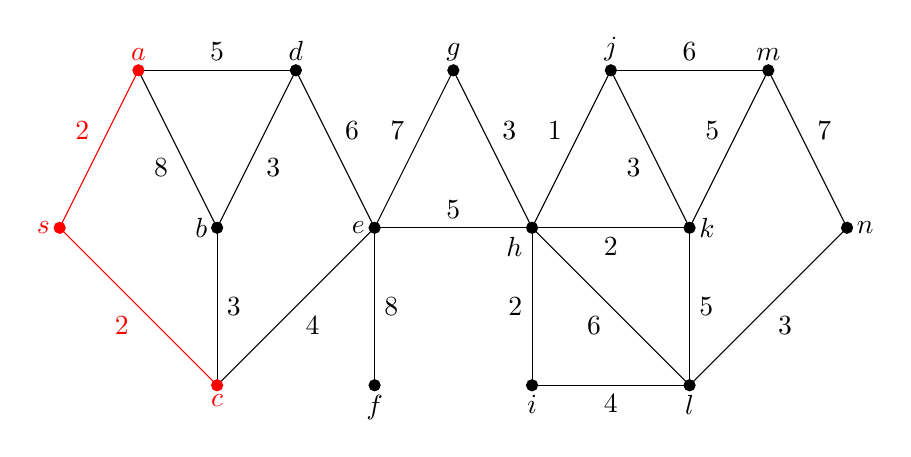
\begin{tikzpicture}

    \coordinate (a) at ( 1, 4);
\coordinate (b) at ( 2, 2);
\coordinate (c) at ( 2, 0);
\coordinate (d) at ( 3, 4);
\coordinate (e) at ( 4, 2);
\coordinate (f) at ( 4, 0);
\coordinate (g) at ( 5, 4);
\coordinate (h) at ( 6, 2);
\coordinate (i) at ( 6, 0);
\coordinate (j) at ( 7, 4);
\coordinate (k) at ( 8, 2);
\coordinate (l) at ( 8, 0);
\coordinate (m) at ( 9, 4);
\coordinate (n) at (10, 2);
\coordinate (s) at ( 0, 2);

    \draw [color = black] (a) -- node [below left]  {$8$} (b);
    \draw [color = black] (a) -- node [above]       {$5$} (d);
    \draw [color = red]   (a) -- node [above left]  {$2$} (s);
    \draw [color = black] (b) -- node [right]       {$3$} (c);
    \draw [color = black] (b) -- node [below right] {$3$} (d);
    \draw [color = black] (c) -- node [below right] {$4$} (e);
    \draw [color = red]   (c) -- node [below left]  {$2$} (s);
    \draw [color = black] (d) -- node [above right] {$6$} (e);
    \draw [color = black] (e) -- node [right]       {$8$} (f);
    \draw [color = black] (e) -- node [above left]  {$7$} (g);
    \draw [color = black] (e) -- node [above]       {$5$} (h);
    \draw [color = black] (g) -- node [above right] {$3$} (h);
    \draw [color = black] (h) -- node [left]        {$2$} (i);
    \draw [color = black] (h) -- node [above left]  {$1$} (j);
    \draw [color = black] (h) -- node [below]       {$2$} (k);
    \draw [color = black] (h) -- node [below left]  {$6$} (l);
    \draw [color = black] (i) -- node [below]       {$4$} (l);
    \draw [color = black] (j) -- node [below left]  {$3$} (k);
    \draw [color = black] (j) -- node [above]       {$6$} (m);
    \draw [color = black] (k) -- node [right]       {$5$} (l);
    \draw [color = black] (k) -- node [above left]  {$5$} (m);
    \draw [color = black] (l) -- node [below right] {$3$} (n);
    \draw [color = black] (m) -- node [above right] {$7$} (n);

    \filldraw [color = red]   (a) circle (2pt) node [above]      {$a$};
    \filldraw [color = black] (b) circle (2pt) node [left]       {$b$};
    \filldraw [color = red]   (c) circle (2pt) node [below]      {$c$};
    \filldraw [color = black] (d) circle (2pt) node [above]      {$d$};
    \filldraw [color = black] (e) circle (2pt) node [left]       {$e$};
    \filldraw [color = black] (f) circle (2pt) node [below]      {$f$};
    \filldraw [color = black] (g) circle (2pt) node [above]      {$g$};
    \filldraw [color = black] (h) circle (2pt) node [below left] {$h$};
    \filldraw [color = black] (i) circle (2pt) node [below]      {$i$};
    \filldraw [color = black] (j) circle (2pt) node [above]      {$j$};
    \filldraw [color = black] (k) circle (2pt) node [right]      {$k$};
    \filldraw [color = black] (l) circle (2pt) node [below]      {$l$};
    \filldraw [color = black] (m) circle (2pt) node [above]      {$m$};
    \filldraw [color = black] (n) circle (2pt) node [right]      {$n$};
    \filldraw [color = red]   (s) circle (2pt) node [left]       {$s$};

\end{tikzpicture}

    \end{center}

    \begin{center}
        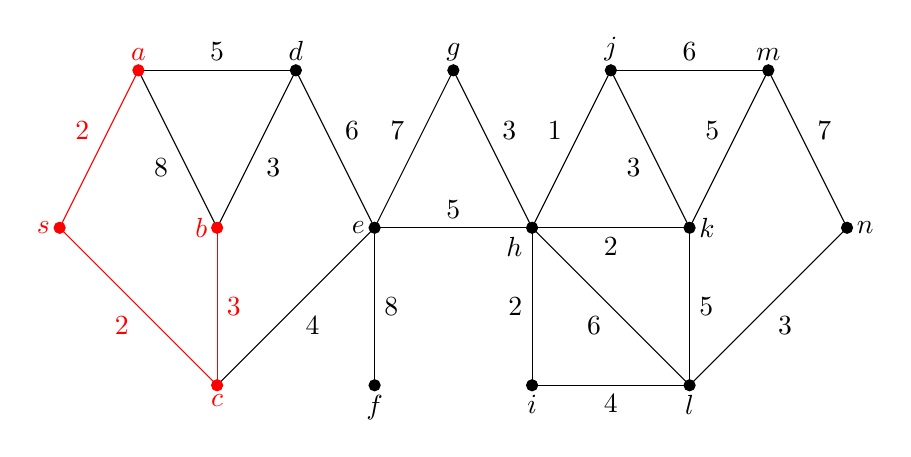
\begin{tikzpicture}

    \coordinate (a) at ( 1, 4);
\coordinate (b) at ( 2, 2);
\coordinate (c) at ( 2, 0);
\coordinate (d) at ( 3, 4);
\coordinate (e) at ( 4, 2);
\coordinate (f) at ( 4, 0);
\coordinate (g) at ( 5, 4);
\coordinate (h) at ( 6, 2);
\coordinate (i) at ( 6, 0);
\coordinate (j) at ( 7, 4);
\coordinate (k) at ( 8, 2);
\coordinate (l) at ( 8, 0);
\coordinate (m) at ( 9, 4);
\coordinate (n) at (10, 2);
\coordinate (s) at ( 0, 2);

    \draw [color = black] (a) -- node [below left]  {$8$} (b);
    \draw [color = black] (a) -- node [above]       {$5$} (d);
    \draw [color = red]   (a) -- node [above left]  {$2$} (s);
    \draw [color = red]   (b) -- node [right]       {$3$} (c);
    \draw [color = black] (b) -- node [below right] {$3$} (d);
    \draw [color = black] (c) -- node [below right] {$4$} (e);
    \draw [color = red]   (c) -- node [below left]  {$2$} (s);
    \draw [color = black] (d) -- node [above right] {$6$} (e);
    \draw [color = black] (e) -- node [right]       {$8$} (f);
    \draw [color = black] (e) -- node [above left]  {$7$} (g);
    \draw [color = black] (e) -- node [above]       {$5$} (h);
    \draw [color = black] (g) -- node [above right] {$3$} (h);
    \draw [color = black] (h) -- node [left]        {$2$} (i);
    \draw [color = black] (h) -- node [above left]  {$1$} (j);
    \draw [color = black] (h) -- node [below]       {$2$} (k);
    \draw [color = black] (h) -- node [below left]  {$6$} (l);
    \draw [color = black] (i) -- node [below]       {$4$} (l);
    \draw [color = black] (j) -- node [below left]  {$3$} (k);
    \draw [color = black] (j) -- node [above]       {$6$} (m);
    \draw [color = black] (k) -- node [right]       {$5$} (l);
    \draw [color = black] (k) -- node [above left]  {$5$} (m);
    \draw [color = black] (l) -- node [below right] {$3$} (n);
    \draw [color = black] (m) -- node [above right] {$7$} (n);

    \filldraw [color = red]   (a) circle (2pt) node [above]      {$a$};
    \filldraw [color = red]   (b) circle (2pt) node [left]       {$b$};
    \filldraw [color = red]   (c) circle (2pt) node [below]      {$c$};
    \filldraw [color = black] (d) circle (2pt) node [above]      {$d$};
    \filldraw [color = black] (e) circle (2pt) node [left]       {$e$};
    \filldraw [color = black] (f) circle (2pt) node [below]      {$f$};
    \filldraw [color = black] (g) circle (2pt) node [above]      {$g$};
    \filldraw [color = black] (h) circle (2pt) node [below left] {$h$};
    \filldraw [color = black] (i) circle (2pt) node [below]      {$i$};
    \filldraw [color = black] (j) circle (2pt) node [above]      {$j$};
    \filldraw [color = black] (k) circle (2pt) node [right]      {$k$};
    \filldraw [color = black] (l) circle (2pt) node [below]      {$l$};
    \filldraw [color = black] (m) circle (2pt) node [above]      {$m$};
    \filldraw [color = black] (n) circle (2pt) node [right]      {$n$};
    \filldraw [color = red]   (s) circle (2pt) node [left]       {$s$};

\end{tikzpicture}

    \end{center}

    \begin{center}
        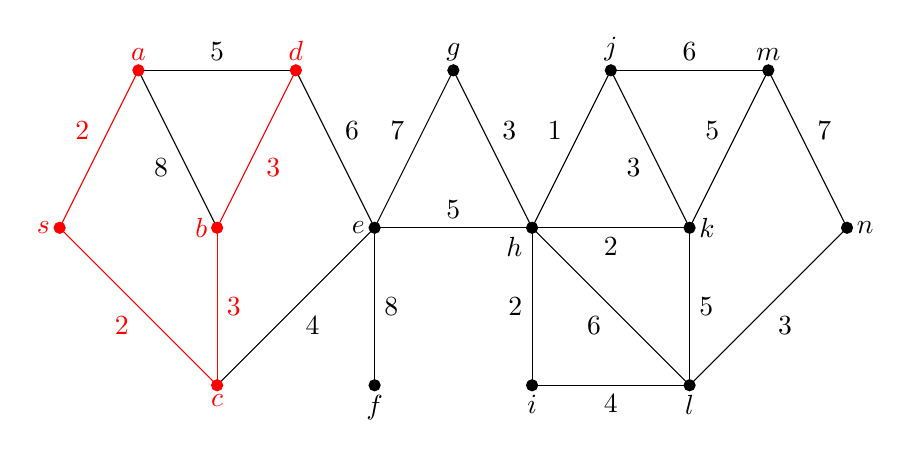
\begin{tikzpicture}

    \coordinate (a) at ( 1, 4);
\coordinate (b) at ( 2, 2);
\coordinate (c) at ( 2, 0);
\coordinate (d) at ( 3, 4);
\coordinate (e) at ( 4, 2);
\coordinate (f) at ( 4, 0);
\coordinate (g) at ( 5, 4);
\coordinate (h) at ( 6, 2);
\coordinate (i) at ( 6, 0);
\coordinate (j) at ( 7, 4);
\coordinate (k) at ( 8, 2);
\coordinate (l) at ( 8, 0);
\coordinate (m) at ( 9, 4);
\coordinate (n) at (10, 2);
\coordinate (s) at ( 0, 2);

    \draw [color = black] (a) -- node [below left]  {$8$} (b);
    \draw [color = black] (a) -- node [above]       {$5$} (d);
    \draw [color = red]   (a) -- node [above left]  {$2$} (s);
    \draw [color = red]   (b) -- node [right]       {$3$} (c);
    \draw [color = red]   (b) -- node [below right] {$3$} (d);
    \draw [color = black] (c) -- node [below right] {$4$} (e);
    \draw [color = red]   (c) -- node [below left]  {$2$} (s);
    \draw [color = black] (d) -- node [above right] {$6$} (e);
    \draw [color = black] (e) -- node [right]       {$8$} (f);
    \draw [color = black] (e) -- node [above left]  {$7$} (g);
    \draw [color = black] (e) -- node [above]       {$5$} (h);
    \draw [color = black] (g) -- node [above right] {$3$} (h);
    \draw [color = black] (h) -- node [left]        {$2$} (i);
    \draw [color = black] (h) -- node [above left]  {$1$} (j);
    \draw [color = black] (h) -- node [below]       {$2$} (k);
    \draw [color = black] (h) -- node [below left]  {$6$} (l);
    \draw [color = black] (i) -- node [below]       {$4$} (l);
    \draw [color = black] (j) -- node [below left]  {$3$} (k);
    \draw [color = black] (j) -- node [above]       {$6$} (m);
    \draw [color = black] (k) -- node [right]       {$5$} (l);
    \draw [color = black] (k) -- node [above left]  {$5$} (m);
    \draw [color = black] (l) -- node [below right] {$3$} (n);
    \draw [color = black] (m) -- node [above right] {$7$} (n);

    \filldraw [color = red]   (a) circle (2pt) node [above]      {$a$};
    \filldraw [color = red]   (b) circle (2pt) node [left]       {$b$};
    \filldraw [color = red]   (c) circle (2pt) node [below]      {$c$};
    \filldraw [color = red]   (d) circle (2pt) node [above]      {$d$};
    \filldraw [color = black] (e) circle (2pt) node [left]       {$e$};
    \filldraw [color = black] (f) circle (2pt) node [below]      {$f$};
    \filldraw [color = black] (g) circle (2pt) node [above]      {$g$};
    \filldraw [color = black] (h) circle (2pt) node [below left] {$h$};
    \filldraw [color = black] (i) circle (2pt) node [below]      {$i$};
    \filldraw [color = black] (j) circle (2pt) node [above]      {$j$};
    \filldraw [color = black] (k) circle (2pt) node [right]      {$k$};
    \filldraw [color = black] (l) circle (2pt) node [below]      {$l$};
    \filldraw [color = black] (m) circle (2pt) node [above]      {$m$};
    \filldraw [color = black] (n) circle (2pt) node [right]      {$n$};
    \filldraw [color = red]   (s) circle (2pt) node [left]       {$s$};

\end{tikzpicture}

    \end{center}

    \begin{center}
        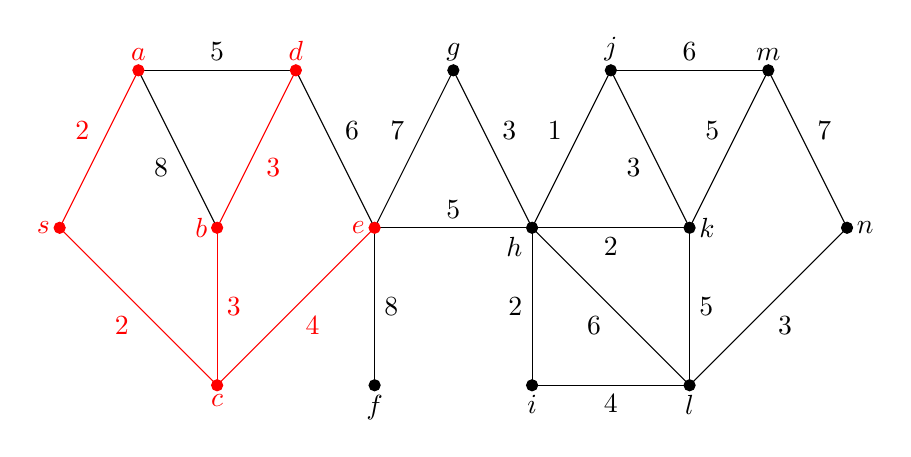
\begin{tikzpicture}

    \coordinate (a) at ( 1, 4);
\coordinate (b) at ( 2, 2);
\coordinate (c) at ( 2, 0);
\coordinate (d) at ( 3, 4);
\coordinate (e) at ( 4, 2);
\coordinate (f) at ( 4, 0);
\coordinate (g) at ( 5, 4);
\coordinate (h) at ( 6, 2);
\coordinate (i) at ( 6, 0);
\coordinate (j) at ( 7, 4);
\coordinate (k) at ( 8, 2);
\coordinate (l) at ( 8, 0);
\coordinate (m) at ( 9, 4);
\coordinate (n) at (10, 2);
\coordinate (s) at ( 0, 2);

    \draw [color = black] (a) -- node [below left]  {$8$} (b);
    \draw [color = black] (a) -- node [above]       {$5$} (d);
    \draw [color = red]   (a) -- node [above left]  {$2$} (s);
    \draw [color = red]   (b) -- node [right]       {$3$} (c);
    \draw [color = red]   (b) -- node [below right] {$3$} (d);
    \draw [color = red]   (c) -- node [below right] {$4$} (e);
    \draw [color = red]   (c) -- node [below left]  {$2$} (s);
    \draw [color = black] (d) -- node [above right] {$6$} (e);
    \draw [color = black] (e) -- node [right]       {$8$} (f);
    \draw [color = black] (e) -- node [above left]  {$7$} (g);
    \draw [color = black] (e) -- node [above]       {$5$} (h);
    \draw [color = black] (g) -- node [above right] {$3$} (h);
    \draw [color = black] (h) -- node [left]        {$2$} (i);
    \draw [color = black] (h) -- node [above left]  {$1$} (j);
    \draw [color = black] (h) -- node [below]       {$2$} (k);
    \draw [color = black] (h) -- node [below left]  {$6$} (l);
    \draw [color = black] (i) -- node [below]       {$4$} (l);
    \draw [color = black] (j) -- node [below left]  {$3$} (k);
    \draw [color = black] (j) -- node [above]       {$6$} (m);
    \draw [color = black] (k) -- node [right]       {$5$} (l);
    \draw [color = black] (k) -- node [above left]  {$5$} (m);
    \draw [color = black] (l) -- node [below right] {$3$} (n);
    \draw [color = black] (m) -- node [above right] {$7$} (n);

    \filldraw [color = red]   (a) circle (2pt) node [above]      {$a$};
    \filldraw [color = red]   (b) circle (2pt) node [left]       {$b$};
    \filldraw [color = red]   (c) circle (2pt) node [below]      {$c$};
    \filldraw [color = red]   (d) circle (2pt) node [above]      {$d$};
    \filldraw [color = red]   (e) circle (2pt) node [left]       {$e$};
    \filldraw [color = black] (f) circle (2pt) node [below]      {$f$};
    \filldraw [color = black] (g) circle (2pt) node [above]      {$g$};
    \filldraw [color = black] (h) circle (2pt) node [below left] {$h$};
    \filldraw [color = black] (i) circle (2pt) node [below]      {$i$};
    \filldraw [color = black] (j) circle (2pt) node [above]      {$j$};
    \filldraw [color = black] (k) circle (2pt) node [right]      {$k$};
    \filldraw [color = black] (l) circle (2pt) node [below]      {$l$};
    \filldraw [color = black] (m) circle (2pt) node [above]      {$m$};
    \filldraw [color = black] (n) circle (2pt) node [right]      {$n$};
    \filldraw [color = red]   (s) circle (2pt) node [left]       {$s$};

\end{tikzpicture}

    \end{center}

    \begin{center}
        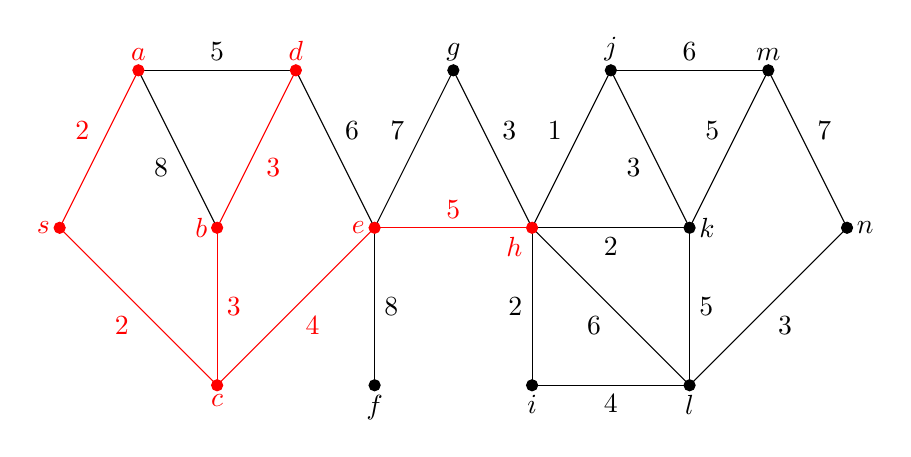
\begin{tikzpicture}

    \coordinate (a) at ( 1, 4);
\coordinate (b) at ( 2, 2);
\coordinate (c) at ( 2, 0);
\coordinate (d) at ( 3, 4);
\coordinate (e) at ( 4, 2);
\coordinate (f) at ( 4, 0);
\coordinate (g) at ( 5, 4);
\coordinate (h) at ( 6, 2);
\coordinate (i) at ( 6, 0);
\coordinate (j) at ( 7, 4);
\coordinate (k) at ( 8, 2);
\coordinate (l) at ( 8, 0);
\coordinate (m) at ( 9, 4);
\coordinate (n) at (10, 2);
\coordinate (s) at ( 0, 2);

    \draw [color = black] (a) -- node [below left]  {$8$} (b);
    \draw [color = black] (a) -- node [above]       {$5$} (d);
    \draw [color = red]   (a) -- node [above left]  {$2$} (s);
    \draw [color = red]   (b) -- node [right]       {$3$} (c);
    \draw [color = red]   (b) -- node [below right] {$3$} (d);
    \draw [color = red]   (c) -- node [below right] {$4$} (e);
    \draw [color = red]   (c) -- node [below left]  {$2$} (s);
    \draw [color = black] (d) -- node [above right] {$6$} (e);
    \draw [color = black] (e) -- node [right]       {$8$} (f);
    \draw [color = black] (e) -- node [above left]  {$7$} (g);
    \draw [color = red]   (e) -- node [above]       {$5$} (h);
    \draw [color = black] (g) -- node [above right] {$3$} (h);
    \draw [color = black] (h) -- node [left]        {$2$} (i);
    \draw [color = black] (h) -- node [above left]  {$1$} (j);
    \draw [color = black] (h) -- node [below]       {$2$} (k);
    \draw [color = black] (h) -- node [below left]  {$6$} (l);
    \draw [color = black] (i) -- node [below]       {$4$} (l);
    \draw [color = black] (j) -- node [below left]  {$3$} (k);
    \draw [color = black] (j) -- node [above]       {$6$} (m);
    \draw [color = black] (k) -- node [right]       {$5$} (l);
    \draw [color = black] (k) -- node [above left]  {$5$} (m);
    \draw [color = black] (l) -- node [below right] {$3$} (n);
    \draw [color = black] (m) -- node [above right] {$7$} (n);

    \filldraw [color = red]   (a) circle (2pt) node [above]      {$a$};
    \filldraw [color = red]   (b) circle (2pt) node [left]       {$b$};
    \filldraw [color = red]   (c) circle (2pt) node [below]      {$c$};
    \filldraw [color = red]   (d) circle (2pt) node [above]      {$d$};
    \filldraw [color = red]   (e) circle (2pt) node [left]       {$e$};
    \filldraw [color = black] (f) circle (2pt) node [below]      {$f$};
    \filldraw [color = black] (g) circle (2pt) node [above]      {$g$};
    \filldraw [color = red]   (h) circle (2pt) node [below left] {$h$};
    \filldraw [color = black] (i) circle (2pt) node [below]      {$i$};
    \filldraw [color = black] (j) circle (2pt) node [above]      {$j$};
    \filldraw [color = black] (k) circle (2pt) node [right]      {$k$};
    \filldraw [color = black] (l) circle (2pt) node [below]      {$l$};
    \filldraw [color = black] (m) circle (2pt) node [above]      {$m$};
    \filldraw [color = black] (n) circle (2pt) node [right]      {$n$};
    \filldraw [color = red]   (s) circle (2pt) node [left]       {$s$};

\end{tikzpicture}

    \end{center}

    \begin{center}
        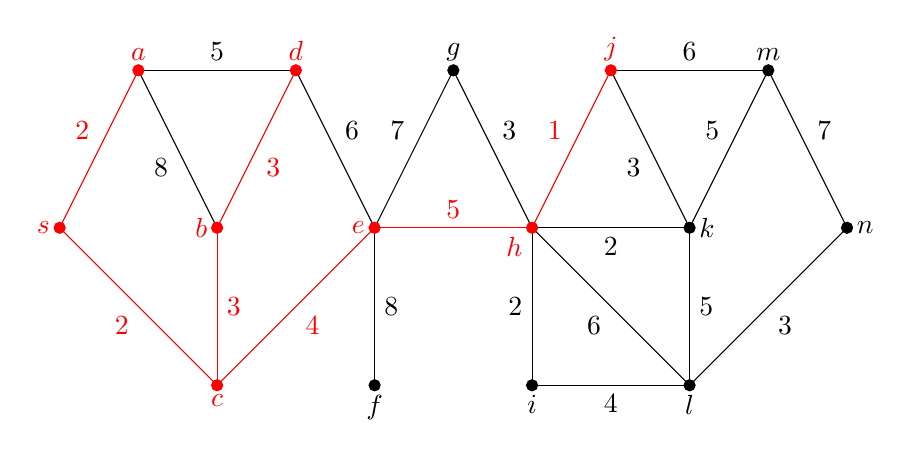
\begin{tikzpicture}

    \coordinate (a) at ( 1, 4);
\coordinate (b) at ( 2, 2);
\coordinate (c) at ( 2, 0);
\coordinate (d) at ( 3, 4);
\coordinate (e) at ( 4, 2);
\coordinate (f) at ( 4, 0);
\coordinate (g) at ( 5, 4);
\coordinate (h) at ( 6, 2);
\coordinate (i) at ( 6, 0);
\coordinate (j) at ( 7, 4);
\coordinate (k) at ( 8, 2);
\coordinate (l) at ( 8, 0);
\coordinate (m) at ( 9, 4);
\coordinate (n) at (10, 2);
\coordinate (s) at ( 0, 2);

    \draw [color = black] (a) -- node [below left]  {$8$} (b);
    \draw [color = black] (a) -- node [above]       {$5$} (d);
    \draw [color = red]   (a) -- node [above left]  {$2$} (s);
    \draw [color = red]   (b) -- node [right]       {$3$} (c);
    \draw [color = red]   (b) -- node [below right] {$3$} (d);
    \draw [color = red]   (c) -- node [below right] {$4$} (e);
    \draw [color = red]   (c) -- node [below left]  {$2$} (s);
    \draw [color = black] (d) -- node [above right] {$6$} (e);
    \draw [color = black] (e) -- node [right]       {$8$} (f);
    \draw [color = black] (e) -- node [above left]  {$7$} (g);
    \draw [color = red]   (e) -- node [above]       {$5$} (h);
    \draw [color = black] (g) -- node [above right] {$3$} (h);
    \draw [color = black] (h) -- node [left]        {$2$} (i);
    \draw [color = red]   (h) -- node [above left]  {$1$} (j);
    \draw [color = black] (h) -- node [below]       {$2$} (k);
    \draw [color = black] (h) -- node [below left]  {$6$} (l);
    \draw [color = black] (i) -- node [below]       {$4$} (l);
    \draw [color = black] (j) -- node [below left]  {$3$} (k);
    \draw [color = black] (j) -- node [above]       {$6$} (m);
    \draw [color = black] (k) -- node [right]       {$5$} (l);
    \draw [color = black] (k) -- node [above left]  {$5$} (m);
    \draw [color = black] (l) -- node [below right] {$3$} (n);
    \draw [color = black] (m) -- node [above right] {$7$} (n);

    \filldraw [color = red]   (a) circle (2pt) node [above]      {$a$};
    \filldraw [color = red]   (b) circle (2pt) node [left]       {$b$};
    \filldraw [color = red]   (c) circle (2pt) node [below]      {$c$};
    \filldraw [color = red]   (d) circle (2pt) node [above]      {$d$};
    \filldraw [color = red]   (e) circle (2pt) node [left]       {$e$};
    \filldraw [color = black] (f) circle (2pt) node [below]      {$f$};
    \filldraw [color = black] (g) circle (2pt) node [above]      {$g$};
    \filldraw [color = red]   (h) circle (2pt) node [below left] {$h$};
    \filldraw [color = black] (i) circle (2pt) node [below]      {$i$};
    \filldraw [color = red]   (j) circle (2pt) node [above]      {$j$};
    \filldraw [color = black] (k) circle (2pt) node [right]      {$k$};
    \filldraw [color = black] (l) circle (2pt) node [below]      {$l$};
    \filldraw [color = black] (m) circle (2pt) node [above]      {$m$};
    \filldraw [color = black] (n) circle (2pt) node [right]      {$n$};
    \filldraw [color = red]   (s) circle (2pt) node [left]       {$s$};

\end{tikzpicture}

    \end{center}

    \begin{center}
        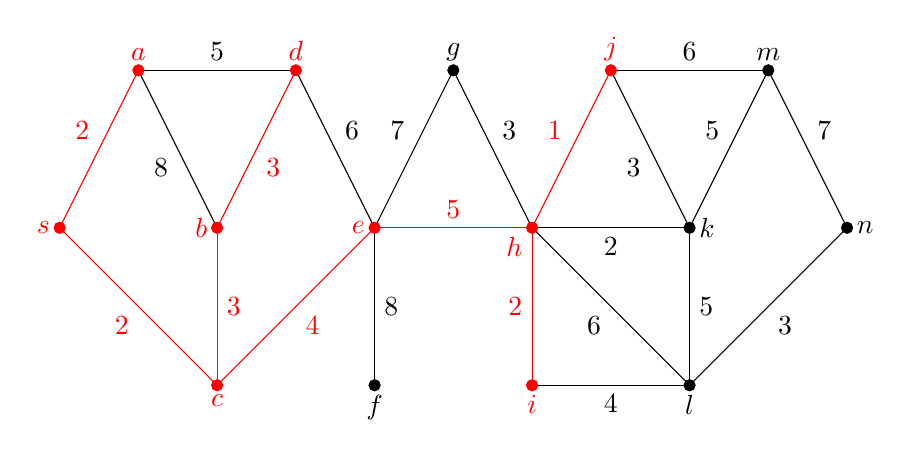
\begin{tikzpicture}

    \coordinate (a) at ( 1, 4);
\coordinate (b) at ( 2, 2);
\coordinate (c) at ( 2, 0);
\coordinate (d) at ( 3, 4);
\coordinate (e) at ( 4, 2);
\coordinate (f) at ( 4, 0);
\coordinate (g) at ( 5, 4);
\coordinate (h) at ( 6, 2);
\coordinate (i) at ( 6, 0);
\coordinate (j) at ( 7, 4);
\coordinate (k) at ( 8, 2);
\coordinate (l) at ( 8, 0);
\coordinate (m) at ( 9, 4);
\coordinate (n) at (10, 2);
\coordinate (s) at ( 0, 2);

    \draw [color = black] (a) -- node [below left]  {$8$} (b);
    \draw [color = black] (a) -- node [above]       {$5$} (d);
    \draw [color = red]   (a) -- node [above left]  {$2$} (s);
    \draw [color = red]   (b) -- node [right]       {$3$} (c);
    \draw [color = red]   (b) -- node [below right] {$3$} (d);
    \draw [color = red]   (c) -- node [below right] {$4$} (e);
    \draw [color = red]   (c) -- node [below left]  {$2$} (s);
    \draw [color = black] (d) -- node [above right] {$6$} (e);
    \draw [color = black] (e) -- node [right]       {$8$} (f);
    \draw [color = black] (e) -- node [above left]  {$7$} (g);
    \draw [color = red]   (e) -- node [above]       {$5$} (h);
    \draw [color = black] (g) -- node [above right] {$3$} (h);
    \draw [color = red]   (h) -- node [left]        {$2$} (i);
    \draw [color = red]   (h) -- node [above left]  {$1$} (j);
    \draw [color = black] (h) -- node [below]       {$2$} (k);
    \draw [color = black] (h) -- node [below left]  {$6$} (l);
    \draw [color = black] (i) -- node [below]       {$4$} (l);
    \draw [color = black] (j) -- node [below left]  {$3$} (k);
    \draw [color = black] (j) -- node [above]       {$6$} (m);
    \draw [color = black] (k) -- node [right]       {$5$} (l);
    \draw [color = black] (k) -- node [above left]  {$5$} (m);
    \draw [color = black] (l) -- node [below right] {$3$} (n);
    \draw [color = black] (m) -- node [above right] {$7$} (n);

    \filldraw [color = red]   (a) circle (2pt) node [above]      {$a$};
    \filldraw [color = red]   (b) circle (2pt) node [left]       {$b$};
    \filldraw [color = red]   (c) circle (2pt) node [below]      {$c$};
    \filldraw [color = red]   (d) circle (2pt) node [above]      {$d$};
    \filldraw [color = red]   (e) circle (2pt) node [left]       {$e$};
    \filldraw [color = black] (f) circle (2pt) node [below]      {$f$};
    \filldraw [color = black] (g) circle (2pt) node [above]      {$g$};
    \filldraw [color = red]   (h) circle (2pt) node [below left] {$h$};
    \filldraw [color = red]   (i) circle (2pt) node [below]      {$i$};
    \filldraw [color = red]   (j) circle (2pt) node [above]      {$j$};
    \filldraw [color = black] (k) circle (2pt) node [right]      {$k$};
    \filldraw [color = black] (l) circle (2pt) node [below]      {$l$};
    \filldraw [color = black] (m) circle (2pt) node [above]      {$m$};
    \filldraw [color = black] (n) circle (2pt) node [right]      {$n$};
    \filldraw [color = red]   (s) circle (2pt) node [left]       {$s$};

\end{tikzpicture}

    \end{center}

    \begin{center}
        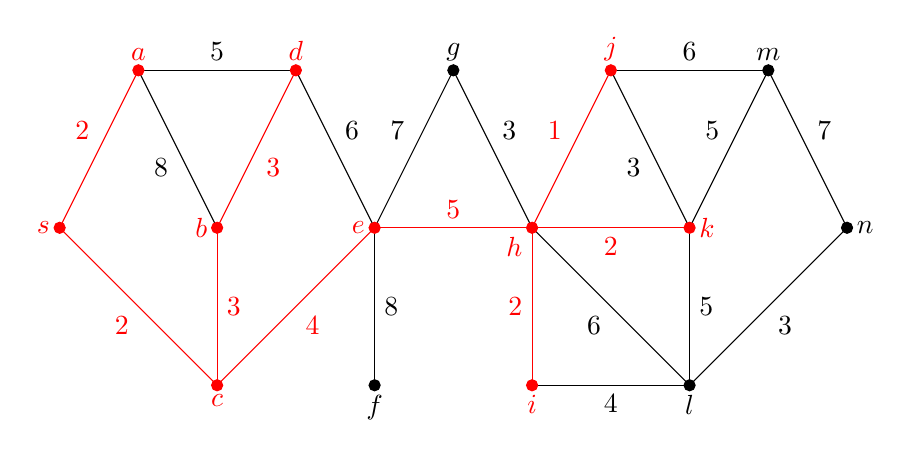
\begin{tikzpicture}

    \coordinate (a) at ( 1, 4);
\coordinate (b) at ( 2, 2);
\coordinate (c) at ( 2, 0);
\coordinate (d) at ( 3, 4);
\coordinate (e) at ( 4, 2);
\coordinate (f) at ( 4, 0);
\coordinate (g) at ( 5, 4);
\coordinate (h) at ( 6, 2);
\coordinate (i) at ( 6, 0);
\coordinate (j) at ( 7, 4);
\coordinate (k) at ( 8, 2);
\coordinate (l) at ( 8, 0);
\coordinate (m) at ( 9, 4);
\coordinate (n) at (10, 2);
\coordinate (s) at ( 0, 2);

    \draw [color = black] (a) -- node [below left]  {$8$} (b);
    \draw [color = black] (a) -- node [above]       {$5$} (d);
    \draw [color = red]   (a) -- node [above left]  {$2$} (s);
    \draw [color = red]   (b) -- node [right]       {$3$} (c);
    \draw [color = red]   (b) -- node [below right] {$3$} (d);
    \draw [color = red]   (c) -- node [below right] {$4$} (e);
    \draw [color = red]   (c) -- node [below left]  {$2$} (s);
    \draw [color = black] (d) -- node [above right] {$6$} (e);
    \draw [color = black] (e) -- node [right]       {$8$} (f);
    \draw [color = black] (e) -- node [above left]  {$7$} (g);
    \draw [color = red]   (e) -- node [above]       {$5$} (h);
    \draw [color = black] (g) -- node [above right] {$3$} (h);
    \draw [color = red]   (h) -- node [left]        {$2$} (i);
    \draw [color = red]   (h) -- node [above left]  {$1$} (j);
    \draw [color = red]   (h) -- node [below]       {$2$} (k);
    \draw [color = black] (h) -- node [below left]  {$6$} (l);
    \draw [color = black] (i) -- node [below]       {$4$} (l);
    \draw [color = black] (j) -- node [below left]  {$3$} (k);
    \draw [color = black] (j) -- node [above]       {$6$} (m);
    \draw [color = black] (k) -- node [right]       {$5$} (l);
    \draw [color = black] (k) -- node [above left]  {$5$} (m);
    \draw [color = black] (l) -- node [below right] {$3$} (n);
    \draw [color = black] (m) -- node [above right] {$7$} (n);

    \filldraw [color = red]   (a) circle (2pt) node [above]      {$a$};
    \filldraw [color = red]   (b) circle (2pt) node [left]       {$b$};
    \filldraw [color = red]   (c) circle (2pt) node [below]      {$c$};
    \filldraw [color = red]   (d) circle (2pt) node [above]      {$d$};
    \filldraw [color = red]   (e) circle (2pt) node [left]       {$e$};
    \filldraw [color = black] (f) circle (2pt) node [below]      {$f$};
    \filldraw [color = black] (g) circle (2pt) node [above]      {$g$};
    \filldraw [color = red]   (h) circle (2pt) node [below left] {$h$};
    \filldraw [color = red]   (i) circle (2pt) node [below]      {$i$};
    \filldraw [color = red]   (j) circle (2pt) node [above]      {$j$};
    \filldraw [color = red]   (k) circle (2pt) node [right]      {$k$};
    \filldraw [color = black] (l) circle (2pt) node [below]      {$l$};
    \filldraw [color = black] (m) circle (2pt) node [above]      {$m$};
    \filldraw [color = black] (n) circle (2pt) node [right]      {$n$};
    \filldraw [color = red]   (s) circle (2pt) node [left]       {$s$};

\end{tikzpicture}

    \end{center}

    \begin{center}
        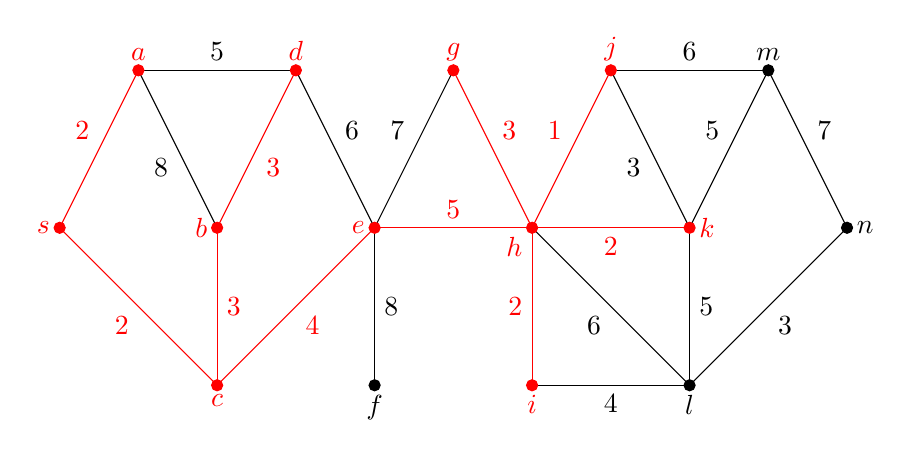
\begin{tikzpicture}

    \coordinate (a) at ( 1, 4);
\coordinate (b) at ( 2, 2);
\coordinate (c) at ( 2, 0);
\coordinate (d) at ( 3, 4);
\coordinate (e) at ( 4, 2);
\coordinate (f) at ( 4, 0);
\coordinate (g) at ( 5, 4);
\coordinate (h) at ( 6, 2);
\coordinate (i) at ( 6, 0);
\coordinate (j) at ( 7, 4);
\coordinate (k) at ( 8, 2);
\coordinate (l) at ( 8, 0);
\coordinate (m) at ( 9, 4);
\coordinate (n) at (10, 2);
\coordinate (s) at ( 0, 2);

    \draw [color = black] (a) -- node [below left]  {$8$} (b);
    \draw [color = black] (a) -- node [above]       {$5$} (d);
    \draw [color = red]   (a) -- node [above left]  {$2$} (s);
    \draw [color = red]   (b) -- node [right]       {$3$} (c);
    \draw [color = red]   (b) -- node [below right] {$3$} (d);
    \draw [color = red]   (c) -- node [below right] {$4$} (e);
    \draw [color = red]   (c) -- node [below left]  {$2$} (s);
    \draw [color = black] (d) -- node [above right] {$6$} (e);
    \draw [color = black] (e) -- node [right]       {$8$} (f);
    \draw [color = black] (e) -- node [above left]  {$7$} (g);
    \draw [color = red]   (e) -- node [above]       {$5$} (h);
    \draw [color = red]   (g) -- node [above right] {$3$} (h);
    \draw [color = red]   (h) -- node [left]        {$2$} (i);
    \draw [color = red]   (h) -- node [above left]  {$1$} (j);
    \draw [color = red]   (h) -- node [below]       {$2$} (k);
    \draw [color = black] (h) -- node [below left]  {$6$} (l);
    \draw [color = black] (i) -- node [below]       {$4$} (l);
    \draw [color = black] (j) -- node [below left]  {$3$} (k);
    \draw [color = black] (j) -- node [above]       {$6$} (m);
    \draw [color = black] (k) -- node [right]       {$5$} (l);
    \draw [color = black] (k) -- node [above left]  {$5$} (m);
    \draw [color = black] (l) -- node [below right] {$3$} (n);
    \draw [color = black] (m) -- node [above right] {$7$} (n);

    \filldraw [color = red]   (a) circle (2pt) node [above]      {$a$};
    \filldraw [color = red]   (b) circle (2pt) node [left]       {$b$};
    \filldraw [color = red]   (c) circle (2pt) node [below]      {$c$};
    \filldraw [color = red]   (d) circle (2pt) node [above]      {$d$};
    \filldraw [color = red]   (e) circle (2pt) node [left]       {$e$};
    \filldraw [color = black] (f) circle (2pt) node [below]      {$f$};
    \filldraw [color = red]   (g) circle (2pt) node [above]      {$g$};
    \filldraw [color = red]   (h) circle (2pt) node [below left] {$h$};
    \filldraw [color = red]   (i) circle (2pt) node [below]      {$i$};
    \filldraw [color = red]   (j) circle (2pt) node [above]      {$j$};
    \filldraw [color = red]   (k) circle (2pt) node [right]      {$k$};
    \filldraw [color = black] (l) circle (2pt) node [below]      {$l$};
    \filldraw [color = black] (m) circle (2pt) node [above]      {$m$};
    \filldraw [color = black] (n) circle (2pt) node [right]      {$n$};
    \filldraw [color = red]   (s) circle (2pt) node [left]       {$s$};

\end{tikzpicture}

    \end{center}

    \begin{center}
        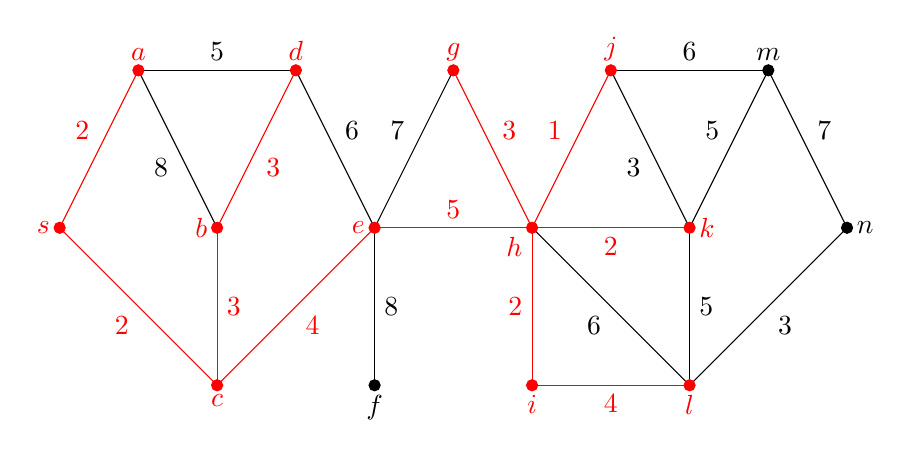
\begin{tikzpicture}

    \coordinate (a) at ( 1, 4);
\coordinate (b) at ( 2, 2);
\coordinate (c) at ( 2, 0);
\coordinate (d) at ( 3, 4);
\coordinate (e) at ( 4, 2);
\coordinate (f) at ( 4, 0);
\coordinate (g) at ( 5, 4);
\coordinate (h) at ( 6, 2);
\coordinate (i) at ( 6, 0);
\coordinate (j) at ( 7, 4);
\coordinate (k) at ( 8, 2);
\coordinate (l) at ( 8, 0);
\coordinate (m) at ( 9, 4);
\coordinate (n) at (10, 2);
\coordinate (s) at ( 0, 2);

    \draw [color = black] (a) -- node [below left]  {$8$} (b);
    \draw [color = black] (a) -- node [above]       {$5$} (d);
    \draw [color = red]   (a) -- node [above left]  {$2$} (s);
    \draw [color = red]   (b) -- node [right]       {$3$} (c);
    \draw [color = red]   (b) -- node [below right] {$3$} (d);
    \draw [color = red]   (c) -- node [below right] {$4$} (e);
    \draw [color = red]   (c) -- node [below left]  {$2$} (s);
    \draw [color = black] (d) -- node [above right] {$6$} (e);
    \draw [color = black] (e) -- node [right]       {$8$} (f);
    \draw [color = black] (e) -- node [above left]  {$7$} (g);
    \draw [color = red]   (e) -- node [above]       {$5$} (h);
    \draw [color = red]   (g) -- node [above right] {$3$} (h);
    \draw [color = red]   (h) -- node [left]        {$2$} (i);
    \draw [color = red]   (h) -- node [above left]  {$1$} (j);
    \draw [color = red]   (h) -- node [below]       {$2$} (k);
    \draw [color = black] (h) -- node [below left]  {$6$} (l);
    \draw [color = red]   (i) -- node [below]       {$4$} (l);
    \draw [color = black] (j) -- node [below left]  {$3$} (k);
    \draw [color = black] (j) -- node [above]       {$6$} (m);
    \draw [color = black] (k) -- node [right]       {$5$} (l);
    \draw [color = black] (k) -- node [above left]  {$5$} (m);
    \draw [color = black] (l) -- node [below right] {$3$} (n);
    \draw [color = black] (m) -- node [above right] {$7$} (n);

    \filldraw [color = red]   (a) circle (2pt) node [above]      {$a$};
    \filldraw [color = red]   (b) circle (2pt) node [left]       {$b$};
    \filldraw [color = red]   (c) circle (2pt) node [below]      {$c$};
    \filldraw [color = red]   (d) circle (2pt) node [above]      {$d$};
    \filldraw [color = red]   (e) circle (2pt) node [left]       {$e$};
    \filldraw [color = black] (f) circle (2pt) node [below]      {$f$};
    \filldraw [color = red]   (g) circle (2pt) node [above]      {$g$};
    \filldraw [color = red]   (h) circle (2pt) node [below left] {$h$};
    \filldraw [color = red]   (i) circle (2pt) node [below]      {$i$};
    \filldraw [color = red]   (j) circle (2pt) node [above]      {$j$};
    \filldraw [color = red]   (k) circle (2pt) node [right]      {$k$};
    \filldraw [color = red]   (l) circle (2pt) node [below]      {$l$};
    \filldraw [color = black] (m) circle (2pt) node [above]      {$m$};
    \filldraw [color = black] (n) circle (2pt) node [right]      {$n$};
    \filldraw [color = red]   (s) circle (2pt) node [left]       {$s$};

\end{tikzpicture}

    \end{center}

    \begin{center}
        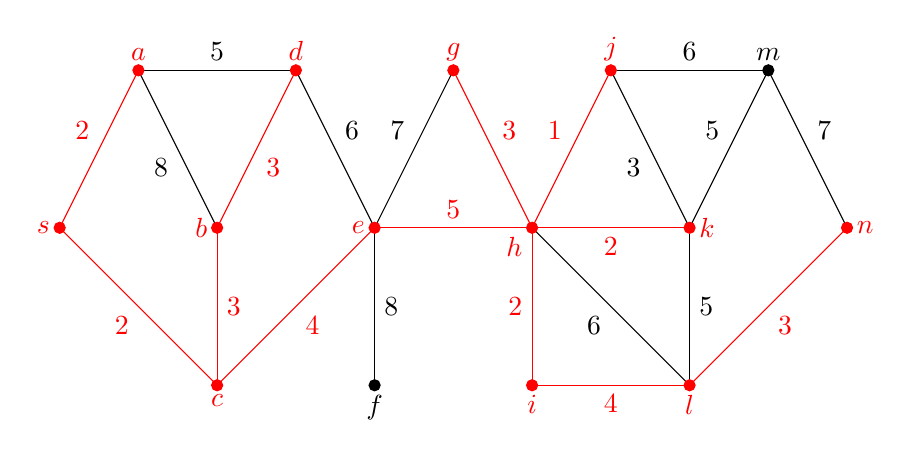
\begin{tikzpicture}

    \coordinate (a) at ( 1, 4);
\coordinate (b) at ( 2, 2);
\coordinate (c) at ( 2, 0);
\coordinate (d) at ( 3, 4);
\coordinate (e) at ( 4, 2);
\coordinate (f) at ( 4, 0);
\coordinate (g) at ( 5, 4);
\coordinate (h) at ( 6, 2);
\coordinate (i) at ( 6, 0);
\coordinate (j) at ( 7, 4);
\coordinate (k) at ( 8, 2);
\coordinate (l) at ( 8, 0);
\coordinate (m) at ( 9, 4);
\coordinate (n) at (10, 2);
\coordinate (s) at ( 0, 2);

    \draw [color = black] (a) -- node [below left]  {$8$} (b);
    \draw [color = black] (a) -- node [above]       {$5$} (d);
    \draw [color = red]   (a) -- node [above left]  {$2$} (s);
    \draw [color = red]   (b) -- node [right]       {$3$} (c);
    \draw [color = red]   (b) -- node [below right] {$3$} (d);
    \draw [color = red]   (c) -- node [below right] {$4$} (e);
    \draw [color = red]   (c) -- node [below left]  {$2$} (s);
    \draw [color = black] (d) -- node [above right] {$6$} (e);
    \draw [color = black] (e) -- node [right]       {$8$} (f);
    \draw [color = black] (e) -- node [above left]  {$7$} (g);
    \draw [color = red]   (e) -- node [above]       {$5$} (h);
    \draw [color = red]   (g) -- node [above right] {$3$} (h);
    \draw [color = red]   (h) -- node [left]        {$2$} (i);
    \draw [color = red]   (h) -- node [above left]  {$1$} (j);
    \draw [color = red]   (h) -- node [below]       {$2$} (k);
    \draw [color = black] (h) -- node [below left]  {$6$} (l);
    \draw [color = red]   (i) -- node [below]       {$4$} (l);
    \draw [color = black] (j) -- node [below left]  {$3$} (k);
    \draw [color = black] (j) -- node [above]       {$6$} (m);
    \draw [color = black] (k) -- node [right]       {$5$} (l);
    \draw [color = black] (k) -- node [above left]  {$5$} (m);
    \draw [color = red]   (l) -- node [below right] {$3$} (n);
    \draw [color = black] (m) -- node [above right] {$7$} (n);

    \filldraw [color = red]   (a) circle (2pt) node [above]      {$a$};
    \filldraw [color = red]   (b) circle (2pt) node [left]       {$b$};
    \filldraw [color = red]   (c) circle (2pt) node [below]      {$c$};
    \filldraw [color = red]   (d) circle (2pt) node [above]      {$d$};
    \filldraw [color = red]   (e) circle (2pt) node [left]       {$e$};
    \filldraw [color = black] (f) circle (2pt) node [below]      {$f$};
    \filldraw [color = red]   (g) circle (2pt) node [above]      {$g$};
    \filldraw [color = red]   (h) circle (2pt) node [below left] {$h$};
    \filldraw [color = red]   (i) circle (2pt) node [below]      {$i$};
    \filldraw [color = red]   (j) circle (2pt) node [above]      {$j$};
    \filldraw [color = red]   (k) circle (2pt) node [right]      {$k$};
    \filldraw [color = red]   (l) circle (2pt) node [below]      {$l$};
    \filldraw [color = black] (m) circle (2pt) node [above]      {$m$};
    \filldraw [color = red]   (n) circle (2pt) node [right]      {$n$};
    \filldraw [color = red]   (s) circle (2pt) node [left]       {$s$};

\end{tikzpicture}

    \end{center}

    \begin{center}
        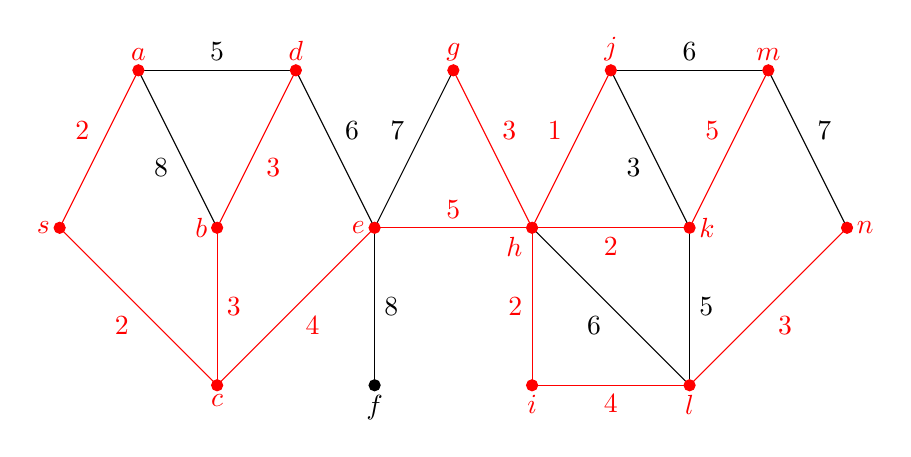
\begin{tikzpicture}

    \coordinate (a) at ( 1, 4);
\coordinate (b) at ( 2, 2);
\coordinate (c) at ( 2, 0);
\coordinate (d) at ( 3, 4);
\coordinate (e) at ( 4, 2);
\coordinate (f) at ( 4, 0);
\coordinate (g) at ( 5, 4);
\coordinate (h) at ( 6, 2);
\coordinate (i) at ( 6, 0);
\coordinate (j) at ( 7, 4);
\coordinate (k) at ( 8, 2);
\coordinate (l) at ( 8, 0);
\coordinate (m) at ( 9, 4);
\coordinate (n) at (10, 2);
\coordinate (s) at ( 0, 2);

    \draw [color = black] (a) -- node [below left]  {$8$} (b);
    \draw [color = black] (a) -- node [above]       {$5$} (d);
    \draw [color = red]   (a) -- node [above left]  {$2$} (s);
    \draw [color = red]   (b) -- node [right]       {$3$} (c);
    \draw [color = red]   (b) -- node [below right] {$3$} (d);
    \draw [color = red]   (c) -- node [below right] {$4$} (e);
    \draw [color = red]   (c) -- node [below left]  {$2$} (s);
    \draw [color = black] (d) -- node [above right] {$6$} (e);
    \draw [color = black] (e) -- node [right]       {$8$} (f);
    \draw [color = black] (e) -- node [above left]  {$7$} (g);
    \draw [color = red]   (e) -- node [above]       {$5$} (h);
    \draw [color = red]   (g) -- node [above right] {$3$} (h);
    \draw [color = red]   (h) -- node [left]        {$2$} (i);
    \draw [color = red]   (h) -- node [above left]  {$1$} (j);
    \draw [color = red]   (h) -- node [below]       {$2$} (k);
    \draw [color = black] (h) -- node [below left]  {$6$} (l);
    \draw [color = red]   (i) -- node [below]       {$4$} (l);
    \draw [color = black] (j) -- node [below left]  {$3$} (k);
    \draw [color = black] (j) -- node [above]       {$6$} (m);
    \draw [color = black] (k) -- node [right]       {$5$} (l);
    \draw [color = red]   (k) -- node [above left]  {$5$} (m);
    \draw [color = red]   (l) -- node [below right] {$3$} (n);
    \draw [color = black] (m) -- node [above right] {$7$} (n);

    \filldraw [color = red]   (a) circle (2pt) node [above]      {$a$};
    \filldraw [color = red]   (b) circle (2pt) node [left]       {$b$};
    \filldraw [color = red]   (c) circle (2pt) node [below]      {$c$};
    \filldraw [color = red]   (d) circle (2pt) node [above]      {$d$};
    \filldraw [color = red]   (e) circle (2pt) node [left]       {$e$};
    \filldraw [color = black] (f) circle (2pt) node [below]      {$f$};
    \filldraw [color = red]   (g) circle (2pt) node [above]      {$g$};
    \filldraw [color = red]   (h) circle (2pt) node [below left] {$h$};
    \filldraw [color = red]   (i) circle (2pt) node [below]      {$i$};
    \filldraw [color = red]   (j) circle (2pt) node [above]      {$j$};
    \filldraw [color = red]   (k) circle (2pt) node [right]      {$k$};
    \filldraw [color = red]   (l) circle (2pt) node [below]      {$l$};
    \filldraw [color = red]   (m) circle (2pt) node [above]      {$m$};
    \filldraw [color = red]   (n) circle (2pt) node [right]      {$n$};
    \filldraw [color = red]   (s) circle (2pt) node [left]       {$s$};

\end{tikzpicture}

    \end{center}

    \begin{center}
        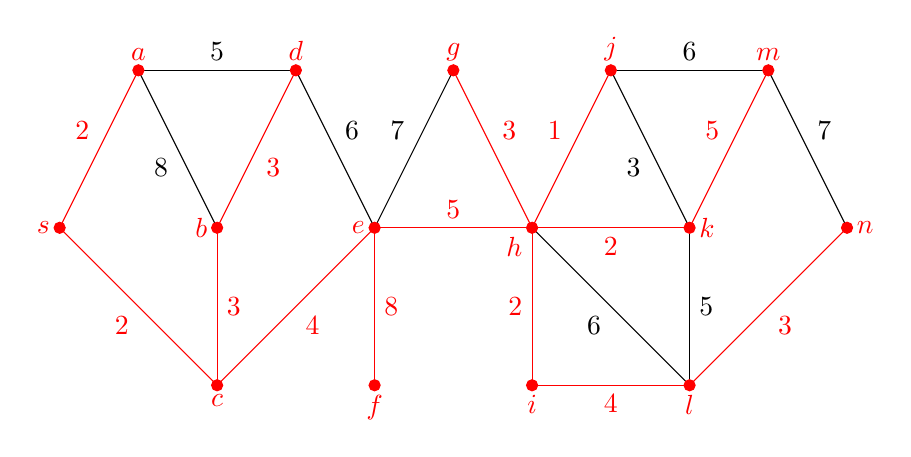
\begin{tikzpicture}

    \coordinate (a) at ( 1, 4);
\coordinate (b) at ( 2, 2);
\coordinate (c) at ( 2, 0);
\coordinate (d) at ( 3, 4);
\coordinate (e) at ( 4, 2);
\coordinate (f) at ( 4, 0);
\coordinate (g) at ( 5, 4);
\coordinate (h) at ( 6, 2);
\coordinate (i) at ( 6, 0);
\coordinate (j) at ( 7, 4);
\coordinate (k) at ( 8, 2);
\coordinate (l) at ( 8, 0);
\coordinate (m) at ( 9, 4);
\coordinate (n) at (10, 2);
\coordinate (s) at ( 0, 2);

    \draw [color = black] (a) -- node [below left]  {$8$} (b);
    \draw [color = black] (a) -- node [above]       {$5$} (d);
    \draw [color = red]   (a) -- node [above left]  {$2$} (s);
    \draw [color = red]   (b) -- node [right]       {$3$} (c);
    \draw [color = red]   (b) -- node [below right] {$3$} (d);
    \draw [color = red]   (c) -- node [below right] {$4$} (e);
    \draw [color = red]   (c) -- node [below left]  {$2$} (s);
    \draw [color = black] (d) -- node [above right] {$6$} (e);
    \draw [color = red]   (e) -- node [right]       {$8$} (f);
    \draw [color = black] (e) -- node [above left]  {$7$} (g);
    \draw [color = red]   (e) -- node [above]       {$5$} (h);
    \draw [color = red]   (g) -- node [above right] {$3$} (h);
    \draw [color = red]   (h) -- node [left]        {$2$} (i);
    \draw [color = red]   (h) -- node [above left]  {$1$} (j);
    \draw [color = red]   (h) -- node [below]       {$2$} (k);
    \draw [color = black] (h) -- node [below left]  {$6$} (l);
    \draw [color = red]   (i) -- node [below]       {$4$} (l);
    \draw [color = black] (j) -- node [below left]  {$3$} (k);
    \draw [color = black] (j) -- node [above]       {$6$} (m);
    \draw [color = black] (k) -- node [right]       {$5$} (l);
    \draw [color = red]   (k) -- node [above left]  {$5$} (m);
    \draw [color = red]   (l) -- node [below right] {$3$} (n);
    \draw [color = black] (m) -- node [above right] {$7$} (n);

    \filldraw [color = red] (a) circle (2pt) node [above]      {$a$};
    \filldraw [color = red] (b) circle (2pt) node [left]       {$b$};
    \filldraw [color = red] (c) circle (2pt) node [below]      {$c$};
    \filldraw [color = red] (d) circle (2pt) node [above]      {$d$};
    \filldraw [color = red] (e) circle (2pt) node [left]       {$e$};
    \filldraw [color = red] (f) circle (2pt) node [below]      {$f$};
    \filldraw [color = red] (g) circle (2pt) node [above]      {$g$};
    \filldraw [color = red] (h) circle (2pt) node [below left] {$h$};
    \filldraw [color = red] (i) circle (2pt) node [below]      {$i$};
    \filldraw [color = red] (j) circle (2pt) node [above]      {$j$};
    \filldraw [color = red] (k) circle (2pt) node [right]      {$k$};
    \filldraw [color = red] (l) circle (2pt) node [below]      {$l$};
    \filldraw [color = red] (m) circle (2pt) node [above]      {$m$};
    \filldraw [color = red] (n) circle (2pt) node [right]      {$n$};
    \filldraw [color = red] (s) circle (2pt) node [left]       {$s$};

\end{tikzpicture}

    \end{center}

\end{enumerate}

\end{solution}

% -------------------------------------------------------------------------------- %
